% !TEX program = xelatex
\documentclass[fontset=windows, 12pt, a4paper]{ctexart}

\usepackage[a4paper, top=2.5cm, bottom=2.5cm, left=2.5cm, right=2.5cm]{geometry}
\usepackage{amsmath,amssymb}
\usepackage{booktabs}
\usepackage{array}
\usepackage{longtable}
\usepackage{xcolor}
\usepackage{graphicx}
\usepackage{float}
\usepackage{listings}
\usepackage{fancyhdr}
\usepackage{titlesec}
\usepackage{pdfpages}

\IfFontExistsTF{Times New Roman}{\setmainfont{Times New Roman}}{}
\IfFontExistsTF{Consolas}{\setmonofont{Consolas}}{}
\newfontfamily\circlednumberfont{SimSun}

\linespread{1.483}
\setlength{\parindent}{2em}
% 正文段落不跨页，避免完整句子在页末被截断。
\interlinepenalty=10000
\widowpenalty=10000
\clubpenalty=10000
\displaywidowpenalty=10000
\setlength{\textfloatsep}{10pt plus 2pt minus 2pt}
\setlength{\intextsep}{8pt plus 2pt minus 2pt}
\setlength{\floatsep}{8pt plus 2pt minus 2pt}

\ctexset{
  section/number       = \arabic{section},
  subsection/number    = \arabic{section}.\arabic{subsection},
  subsubsection/number = \arabic{section}.\arabic{subsection}.\arabic{subsubsection},
}
\setcounter{tocdepth}{2}

\titleformat{\section}
  {\centering\fontsize{16pt}{19.2pt}\heiti\bfseries}
  {\arabic{section}}{1em}{}
\titleformat{\subsection}
  {\fontsize{14pt}{16.8pt}\heiti\bfseries}
  {\arabic{section}.\arabic{subsection}}{1em}{}
\titleformat{\subsubsection}
  {\fontsize{12pt}{14.4pt}\heiti\bfseries}
  {\arabic{section}.\arabic{subsection}.\arabic{subsubsection}}{1em}{}
\titlespacing{\section}       {0pt}{1.8em}{1.0em}
\titlespacing{\subsection}    {0pt}{1.25em}{0.65em}
\titlespacing{\subsubsection} {0pt}{0.9em}{0.4em}

\lstset{
  basicstyle=\ttfamily\small,
  backgroundcolor=\color{black!3},
  frame=single,
  framesep=6pt,
  rulecolor=\color{black!30},
  framerule=0.8pt,
  breaklines=true,
  showstringspaces=false,
  columns=fullflexible,
  keepspaces=true,
}

\pagestyle{fancy}
\setlength{\headheight}{14.5pt}
\fancyhf{}
\fancyhead[C]{\fontsize{10.5pt}{12.6pt}数学建模竞赛论文}
\fancyfoot[C]{\thepage}
\renewcommand{\headrulewidth}{0.4pt}

\newcommand{\papertitle}[1]{%
  \thispagestyle{fancy}%
  \begin{center}
    {\fontsize{22pt}{26.4pt}\heiti\bfseries #1}
  \end{center}
  \vspace{0.55em}
}

\newcommand{\abstractcn}[2]{%
  \begin{center}{\fontsize{14pt}{16.8pt}\heiti\bfseries 摘\hspace{2em}要}\end{center}
  \vspace{0.3em}
  #1\par
  \vspace{0.3em}
  \noindent{\heiti\bfseries 关键词：}#2\par
  \newpage
}

\newcommand{\referencescn}{%
  \begin{thebibliography}{99}
\footnotesize
\linespread{1.0}\selectfont
\setlength{\itemsep}{0.12em}
\setlength{\parskip}{0pt}
\bibitem{Mousavi2020FPCF} Mousavi S F, Hashemabadi S H, Jamali J. Calculation of geometric flow profile correction factor for ultrasonic flow meter using semi-3D simulation technique[J]. Ultrasonics, 2020, 106: 106165.
\bibitem{Sakhavi2022GeneralizedProfile} Sakhavi N, Nouri N M. Generalized velocity profile evaluation of multipath ultrasonic phased array flowmeter[J]. Measurement, 2022, 187: 110302.
\bibitem{Gryshanova2023CorrectionFactor} Gryshanova I, Rak A, Korobko I. The investigation of the correction factor for ultrasonic flow meters[J]. Measurement, 2023, 219: 113326.
\bibitem{Li2023MLInUse} Li M, Li Z, Li C. In-use measurement of ultrasonic flowmeter based on machine learning[J]. Measurement, 2023, 223: 113721.
\bibitem{Qin2016ProfileIdentification} Qin L, Hu L, Mao K, Chen W, Fu X. Flow profile identification with multipath transducers[J]. Flow Measurement and Instrumentation, 2016, 52: 148--156.
\bibitem{Papathanasiou2022FlowDC} Papathanasiou P, Kissling B, Berberig O, Kumar V, Rohner A, Bezdek M. Flow disturbance compensation calculated with flow simulations for ultrasonic clamp-on flowmeters with optimized path arrangement[J]. Flow Measurement and Instrumentation, 2022, 85: 102167.
\bibitem{Zhao2014ANN} Zhao H, Peng L, Takahashi T, Hayashi T, Shimizu K, Yamamoto T. ANN based data integration for multi-path ultrasonic flowmeter[J]. IEEE Sensors Journal, 2014, 14(2): 362--370.
\bibitem{Zhao2014CFD} Zhao H, Peng L, Stephane S A, Ishikawa H, Shimizu K, Takamoto M. CFD aided investigation of multipath ultrasonic gas flow meter performance under complex flow profile[J]. IEEE Sensors Journal, 2014, 14(3): 897--907.
\bibitem{Scholkopf2002LearningKernels} Sch\"olkopf B, Smola A J. Learning with Kernels: Support Vector Machines, Regularization, Optimization, and Beyond[M]. Cambridge, MA: MIT Press, 2002.
\bibitem{Li2025VMDDenoising} Li Z, Liao H, Chen G, Liang H, Zhao L, Sun H. VMD-based adaptive ultrasonic flowmeter echo signal denoising algorithm[J]. Flow Measurement and Instrumentation, 2025, 106: 103044.
\bibitem{Cai2025PhysConstrainedGAN} Cai H, Zhang H, Zhou K, Lin K, Wang X, Liu W, Tang X Y. Physically constrained generative adversarial network data augmentation method for multichannel ultrasonic flowmeters of natural gas[J]. Flow Measurement and Instrumentation, 2025, 102: 102804.
\bibitem{JinUpstreamDisturbance} 金少杰, 牛振雨, 张丽稳, 等. 上游扰流条件对超声波流量计准确度的影响研究[J/OL]. 中国测试, 网络首发, 2025-09-17.
\bibitem{SuUnderdevelopedFlow} 苏杰. 多声道气体超声流量计非充分发展流条件下的仿真结果量化和实验研究[J]. 工业计量, 2024(增刊).
\bibitem{HuangClampOnOil} 黄恩扬. 油品外夹式超声波流量计计量误差研究[D]. 中国石油大学, 2024.
\bibitem{XiangMultipathIntegration} 相诺林. 高精度多声道超声波流量计积分方法及影响因素研究[D]. 河北大学, 2023.
\bibitem{OpenAICodex2026} OpenAI. ChatGPT（具体模型名称以客户端实际显示为准）[EB/OL]. OpenAI, 2026-07-11; OpenAI Codex Desktop（客户端未显示具体模型和构建号）[EB/OL]. OpenAI, 2026-07-08 至 2026-07-12.
\end{thebibliography}
%
}

\newcommand{\appendixcn}{%
  \section*{附录 A\quad 支撑材料与完整源程序}%
  本附录对应最终提交支撑包，内容分为支撑材料目录、完整文件清单、源程序说明和复现顺序。赛题附件 1 至附件 7 属于赛事统一提供的数据，按规范不重复放入支撑包；复现时应将原始目录“A题 (1)”放在支撑包根目录。附录 B 逐行收录建模使用的全部 11 个 Python 文件，不包含废弃模型、文档转换或临时绘图脚本。

\subsection*{A.1 支撑材料目录结构}

\begingroup
\small
\setlength{\tabcolsep}{4pt}
\begin{longtable}{p{0.31\textwidth}p{0.60\textwidth}}
\toprule
目录或文件 & 内容与用途 \\
\midrule
\endfirsthead
\toprule
目录或文件 & 内容与用途 \\
\midrule
\endhead
{\ttfamily\raggedright code/paper\_\allowbreak appendix/\par} & 四个问题、模型演进、最终后校准和官方指标复验所需的 11 个完整 Python 文件。 \\
\texttt{code/outputs/} & 问题三复跑时可选读取的整组留出失效诊断结果。 \\
\texttt{02\_关键结果数据/} & 基础积分、D0 校准、扰流特征、模型比较、最终提交和失效分析的必要结果。 \\
\texttt{03\_论文采用图表/} & 正文实际使用的 10 幅 PDF 图以及问题四工程图的可编辑 DrawIO 源文件。 \\
\texttt{04\_自主查阅资料/} & 文献理论索引与直接支撑积分、剖面修正、ANN、KRR 和物理约束的关键原文。 \\
\texttt{05\_复验与说明/} & 源码独立复跑记录、官方评价结果、文件哈希、AI 工具使用详情和终审报告。 \\
\texttt{requirements.txt} & Python 第三方依赖清单。 \\
\texttt{README.md} & 支撑包结构、原始附件放置方式和运行入口。 \\
\bottomrule
\end{longtable}
\endgroup

\subsection*{A.2 支撑材料完整文件清单}

下表逐项列出最终压缩包中的全部文件。文件哈希另见支撑包中的 \texttt{05\_复验与说明/文件清单与SHA256.csv}。

% Generated from the final support package. Do not edit by hand.
\begingroup
\scriptsize
\setlength{\tabcolsep}{3pt}
\renewcommand{\arraystretch}{0.92}
\begin{longtable}{p{0.055\textwidth}p{0.19\textwidth}p{0.665\textwidth}}
\toprule
序号 & 类别 & 相对路径 \\
\midrule
\endfirsthead
\toprule
序号 & 类别 & 相对路径 \\
\midrule
\endhead
1 & 关键结果数据 & {\ttfamily\raggedright 02\_\allowbreak{}关键结果数据/\allowbreak{}灵敏度与失效/\allowbreak{}krr\_\allowbreak{}leave\_\allowbreak{}one\_\allowbreak{}group\_\allowbreak{}failure\_\allowbreak{}modes.csv\par} \\
2 & 关键结果数据 & {\ttfamily\raggedright 02\_\allowbreak{}关键结果数据/\allowbreak{}灵敏度与失效/\allowbreak{}krr\_\allowbreak{}leave\_\allowbreak{}one\_\allowbreak{}group\_\allowbreak{}ood\_\allowbreak{}diagnostics.csv\par} \\
3 & 关键结果数据 & {\ttfamily\raggedright 02\_\allowbreak{}关键结果数据/\allowbreak{}灵敏度与失效/\allowbreak{}krr\_\allowbreak{}ood\_\allowbreak{}correlation\_\allowbreak{}sensitivity.csv\par} \\
4 & 关键结果数据 & {\ttfamily\raggedright 02\_\allowbreak{}关键结果数据/\allowbreak{}灵敏度与失效/\allowbreak{}krr\_\allowbreak{}pressure\_\allowbreak{}failure\_\allowbreak{}modes.csv\par} \\
5 & 关键结果数据 & {\ttfamily\raggedright 02\_\allowbreak{}关键结果数据/\allowbreak{}灵敏度与失效/\allowbreak{}krr\_\allowbreak{}pressure\_\allowbreak{}ood\_\allowbreak{}groups.csv\par} \\
6 & 关键结果数据 & {\ttfamily\raggedright 02\_\allowbreak{}关键结果数据/\allowbreak{}问题一\_\allowbreak{}基础积分/\allowbreak{}integration\_\allowbreak{}estimates\_\allowbreak{}long.csv\par} \\
7 & 关键结果数据 & {\ttfamily\raggedright 02\_\allowbreak{}关键结果数据/\allowbreak{}问题一\_\allowbreak{}基础积分/\allowbreak{}integration\_\allowbreak{}metrics\_\allowbreak{}by\_\allowbreak{}disturbed.csv\par} \\
8 & 关键结果数据 & {\ttfamily\raggedright 02\_\allowbreak{}关键结果数据/\allowbreak{}问题一\_\allowbreak{}基础积分/\allowbreak{}integration\_\allowbreak{}metrics\_\allowbreak{}by\_\allowbreak{}flow\_\allowbreak{}point.csv\par} \\
9 & 关键结果数据 & {\ttfamily\raggedright 02\_\allowbreak{}关键结果数据/\allowbreak{}问题一\_\allowbreak{}基础积分/\allowbreak{}integration\_\allowbreak{}overall\_\allowbreak{}metrics.csv\par} \\
10 & 关键结果数据 & {\ttfamily\raggedright 02\_\allowbreak{}关键结果数据/\allowbreak{}问题一\_\allowbreak{}基础积分/\allowbreak{}integration\_\allowbreak{}weights.csv\par} \\
11 & 关键结果数据 & {\ttfamily\raggedright 02\_\allowbreak{}关键结果数据/\allowbreak{}问题三\_\allowbreak{}特征与聚类/\allowbreak{}disturbance\_\allowbreak{}cluster\_\allowbreak{}cross\_\allowbreak{}disturbance.csv\par} \\
12 & 关键结果数据 & {\ttfamily\raggedright 02\_\allowbreak{}关键结果数据/\allowbreak{}问题三\_\allowbreak{}特征与聚类/\allowbreak{}disturbance\_\allowbreak{}cluster\_\allowbreak{}quality.csv\par} \\
13 & 关键结果数据 & {\ttfamily\raggedright 02\_\allowbreak{}关键结果数据/\allowbreak{}问题三\_\allowbreak{}特征与聚类/\allowbreak{}disturbance\_\allowbreak{}feature\_\allowbreak{}importance.csv\par} \\
14 & 关键结果数据 & {\ttfamily\raggedright 02\_\allowbreak{}关键结果数据/\allowbreak{}问题三\_\allowbreak{}特征与聚类/\allowbreak{}disturbance\_\allowbreak{}pca\_\allowbreak{}coordinates.csv\par} \\
15 & 关键结果数据 & {\ttfamily\raggedright 02\_\allowbreak{}关键结果数据/\allowbreak{}问题三\_\allowbreak{}特征与聚类/\allowbreak{}disturbance\_\allowbreak{}pca\_\allowbreak{}explained\_\allowbreak{}variance.csv\par} \\
16 & 关键结果数据 & {\ttfamily\raggedright 02\_\allowbreak{}关键结果数据/\allowbreak{}问题二\_\allowbreak{}D0校准/\allowbreak{}d0\_\allowbreak{}model\_\allowbreak{}by\_\allowbreak{}flow\_\allowbreak{}d0\_\allowbreak{}only.csv\par} \\
17 & 关键结果数据 & {\ttfamily\raggedright 02\_\allowbreak{}关键结果数据/\allowbreak{}问题二\_\allowbreak{}D0校准/\allowbreak{}d0\_\allowbreak{}model\_\allowbreak{}overall\_\allowbreak{}d0\_\allowbreak{}only.csv\par} \\
18 & 关键结果数据 & {\ttfamily\raggedright 02\_\allowbreak{}关键结果数据/\allowbreak{}问题二\_\allowbreak{}D0校准/\allowbreak{}phys6\_\allowbreak{}d0\_\allowbreak{}curve\_\allowbreak{}coefficients\_\allowbreak{}main\_\allowbreak{}split.csv\par} \\
19 & 关键结果数据 & {\ttfamily\raggedright 02\_\allowbreak{}关键结果数据/\allowbreak{}问题四\_\allowbreak{}最终模型/\allowbreak{}d0\_\allowbreak{}rbf\_\allowbreak{}postcalibrated\_\allowbreak{}dual\_\allowbreak{}kernel\_\allowbreak{}krr\_\allowbreak{}candidate\_\allowbreak{}ranking.csv\par} \\
20 & 关键结果数据 & {\ttfamily\raggedright 02\_\allowbreak{}关键结果数据/\allowbreak{}问题四\_\allowbreak{}最终模型/\allowbreak{}d0\_\allowbreak{}rbf\_\allowbreak{}postcalibrated\_\allowbreak{}dual\_\allowbreak{}kernel\_\allowbreak{}krr\_\allowbreak{}evaluation\_\allowbreak{}groups.csv\par} \\
21 & 关键结果数据 & {\ttfamily\raggedright 02\_\allowbreak{}关键结果数据/\allowbreak{}问题四\_\allowbreak{}最终模型/\allowbreak{}d0\_\allowbreak{}rbf\_\allowbreak{}postcalibrated\_\allowbreak{}dual\_\allowbreak{}kernel\_\allowbreak{}krr\_\allowbreak{}evaluation\_\allowbreak{}summary.csv\par} \\
22 & 关键结果数据 & {\ttfamily\raggedright 02\_\allowbreak{}关键结果数据/\allowbreak{}问题四\_\allowbreak{}最终模型/\allowbreak{}d0\_\allowbreak{}rbf\_\allowbreak{}postcalibrated\_\allowbreak{}dual\_\allowbreak{}kernel\_\allowbreak{}krr\_\allowbreak{}evaluation\_\allowbreak{}windows.csv\par} \\
23 & 关键结果数据 & {\ttfamily\raggedright 02\_\allowbreak{}关键结果数据/\allowbreak{}问题四\_\allowbreak{}最终模型/\allowbreak{}d0\_\allowbreak{}rbf\_\allowbreak{}postcalibrated\_\allowbreak{}dual\_\allowbreak{}kernel\_\allowbreak{}krr\_\allowbreak{}model.npz\par} \\
24 & 关键结果数据 & {\ttfamily\raggedright 02\_\allowbreak{}关键结果数据/\allowbreak{}问题四\_\allowbreak{}最终模型/\allowbreak{}d0\_\allowbreak{}rbf\_\allowbreak{}postcalibrated\_\allowbreak{}dual\_\allowbreak{}kernel\_\allowbreak{}krr\_\allowbreak{}model\_\allowbreak{}meta.json\par} \\
25 & 关键结果数据 & {\ttfamily\raggedright 02\_\allowbreak{}关键结果数据/\allowbreak{}问题四\_\allowbreak{}最终模型/\allowbreak{}submission\_\allowbreak{}final.csv\par} \\
26 & 关键结果数据 & {\ttfamily\raggedright 02\_\allowbreak{}关键结果数据/\allowbreak{}问题四\_\allowbreak{}模型比较/\allowbreak{}ann\_\allowbreak{}krr\_\allowbreak{}same\_\allowbreak{}split\_\allowbreak{}assignments.csv\par} \\
27 & 关键结果数据 & {\ttfamily\raggedright 02\_\allowbreak{}关键结果数据/\allowbreak{}问题四\_\allowbreak{}模型比较/\allowbreak{}ann\_\allowbreak{}krr\_\allowbreak{}same\_\allowbreak{}split\_\allowbreak{}comparison.csv\par} \\
28 & 关键结果数据 & {\ttfamily\raggedright 02\_\allowbreak{}关键结果数据/\allowbreak{}问题四\_\allowbreak{}模型比较/\allowbreak{}final\_\allowbreak{}model\_\allowbreak{}evolution\_\allowbreak{}comparison.csv\par} \\
29 & 关键结果数据 & {\ttfamily\raggedright 02\_\allowbreak{}关键结果数据/\allowbreak{}问题四\_\allowbreak{}模型比较/\allowbreak{}fullfit\_\allowbreak{}interpolation\_\allowbreak{}evaluation\_\allowbreak{}summary.csv\par} \\
30 & 关键结果数据 & {\ttfamily\raggedright 02\_\allowbreak{}关键结果数据/\allowbreak{}问题四\_\allowbreak{}模型比较/\allowbreak{}krr\_\allowbreak{}champion\_\allowbreak{}multisplit\_\allowbreak{}metrics.csv\par} \\
31 & 关键结果数据 & {\ttfamily\raggedright 02\_\allowbreak{}关键结果数据/\allowbreak{}问题四\_\allowbreak{}模型比较/\allowbreak{}krr\_\allowbreak{}champion\_\allowbreak{}multisplit\_\allowbreak{}pass\_\allowbreak{}rates.csv\par} \\
32 & 关键结果数据 & {\ttfamily\raggedright 02\_\allowbreak{}关键结果数据/\allowbreak{}问题四\_\allowbreak{}模型比较/\allowbreak{}krr\_\allowbreak{}champion\_\allowbreak{}multisplit\_\allowbreak{}summary.csv\par} \\
33 & 关键结果数据 & {\ttfamily\raggedright 02\_\allowbreak{}关键结果数据/\allowbreak{}问题四\_\allowbreak{}模型比较/\allowbreak{}krr\_\allowbreak{}mainline\_\allowbreak{}ablation\_\allowbreak{}main\_\allowbreak{}validation.csv\par} \\
34 & 关键结果数据 & {\ttfamily\raggedright 02\_\allowbreak{}关键结果数据/\allowbreak{}问题四\_\allowbreak{}模型比较/\allowbreak{}stratified\_\allowbreak{}model\_\allowbreak{}search\_\allowbreak{}best\_\allowbreak{}split.csv\par} \\
35 & 关键结果数据 & {\ttfamily\raggedright 02\_\allowbreak{}关键结果数据/\allowbreak{}问题四\_\allowbreak{}模型比较/\allowbreak{}stratified\_\allowbreak{}model\_\allowbreak{}search\_\allowbreak{}multisplit\_\allowbreak{}summary.csv\par} \\
36 & 关键结果数据 & {\ttfamily\raggedright 02\_\allowbreak{}关键结果数据/\allowbreak{}问题四\_\allowbreak{}模型比较/\allowbreak{}stratified\_\allowbreak{}model\_\allowbreak{}search\_\allowbreak{}pressure\_\allowbreak{}split.csv\par} \\
37 & 论文采用图表 & {\ttfamily\raggedright 03\_\allowbreak{}论文采用图表/\allowbreak{}fig\_\allowbreak{}disturbance\_\allowbreak{}feature\_\allowbreak{}importance.pdf\par} \\
38 & 论文采用图表 & {\ttfamily\raggedright 03\_\allowbreak{}论文采用图表/\allowbreak{}fig\_\allowbreak{}disturbance\_\allowbreak{}pca\_\allowbreak{}clusters.pdf\par} \\
39 & 论文采用图表 & {\ttfamily\raggedright 03\_\allowbreak{}论文采用图表/\allowbreak{}fig\_\allowbreak{}disturbance\_\allowbreak{}profile\_\allowbreak{}representativeness.pdf\par} \\
40 & 论文采用图表 & {\ttfamily\raggedright 03\_\allowbreak{}论文采用图表/\allowbreak{}fig\_\allowbreak{}integration\_\allowbreak{}flow\_\allowbreak{}mae.pdf\par} \\
41 & 论文采用图表 & {\ttfamily\raggedright 03\_\allowbreak{}论文采用图表/\allowbreak{}fig\_\allowbreak{}krr\_\allowbreak{}ablation\_\allowbreak{}metrics.pdf\par} \\
42 & 论文采用图表 & {\ttfamily\raggedright 03\_\allowbreak{}论文采用图表/\allowbreak{}fig\_\allowbreak{}krr\_\allowbreak{}ood\_\allowbreak{}vs\_\allowbreak{}error.pdf\par} \\
43 & 论文采用图表 & {\ttfamily\raggedright 03\_\allowbreak{}论文采用图表/\allowbreak{}fig\_\allowbreak{}leave\_\allowbreak{}one\_\allowbreak{}group\_\allowbreak{}error\_\allowbreak{}heatmap.pdf\par} \\
44 & 论文采用图表 & {\ttfamily\raggedright 03\_\allowbreak{}论文采用图表/\allowbreak{}fig\_\allowbreak{}model\_\allowbreak{}mae\_\allowbreak{}comparison.pdf\par} \\
45 & 论文采用图表 & {\ttfamily\raggedright 03\_\allowbreak{}论文采用图表/\allowbreak{}fig\_\allowbreak{}prediction\_\allowbreak{}consistency.pdf\par} \\
46 & 论文采用图表 & {\ttfamily\raggedright 03\_\allowbreak{}论文采用图表/\allowbreak{}fig\_\allowbreak{}problem4\_\allowbreak{}engineering\_\allowbreak{}pipeline.drawio\par} \\
47 & 论文采用图表 & {\ttfamily\raggedright 03\_\allowbreak{}论文采用图表/\allowbreak{}fig\_\allowbreak{}problem4\_\allowbreak{}engineering\_\allowbreak{}pipeline.pdf\par} \\
48 & 自主查阅资料 & {\ttfamily\raggedright 04\_\allowbreak{}自主查阅资料/\allowbreak{}关键原文/\allowbreak{}ANN\_\allowbreak{}data\_\allowbreak{}integration\_\allowbreak{}for\_\allowbreak{}multipath\_\allowbreak{}ultrasonic\_\allowbreak{}flowmeter.pdf\par} \\
49 & 自主查阅资料 & {\ttfamily\raggedright 04\_\allowbreak{}自主查阅资料/\allowbreak{}关键原文/\allowbreak{}Calculation\_\allowbreak{}geometric\_\allowbreak{}flow\_\allowbreak{}profile\_\allowbreak{}correction\_\allowbreak{}factor.pdf\par} \\
50 & 自主查阅资料 & {\ttfamily\raggedright 04\_\allowbreak{}自主查阅资料/\allowbreak{}关键原文/\allowbreak{}Flow\_\allowbreak{}profile\_\allowbreak{}identification\_\allowbreak{}by\_\allowbreak{}multi\_\allowbreak{}channel\_\allowbreak{}measurements.pdf\par} \\
51 & 自主查阅资料 & {\ttfamily\raggedright 04\_\allowbreak{}自主查阅资料/\allowbreak{}关键原文/\allowbreak{}Generalized\_\allowbreak{}velocity\_\allowbreak{}profile\_\allowbreak{}evaluation.pdf\par} \\
52 & 自主查阅资料 & {\ttfamily\raggedright 04\_\allowbreak{}自主查阅资料/\allowbreak{}关键原文/\allowbreak{}In\_\allowbreak{}use\_\allowbreak{}measurement\_\allowbreak{}based\_\allowbreak{}on\_\allowbreak{}machine\_\allowbreak{}learning.pdf\par} \\
53 & 自主查阅资料 & {\ttfamily\raggedright 04\_\allowbreak{}自主查阅资料/\allowbreak{}关键原文/\allowbreak{}Physically\_\allowbreak{}constrained\_\allowbreak{}GAN\_\allowbreak{}data\_\allowbreak{}augmentation.pdf\par} \\
54 & 自主查阅资料 & {\ttfamily\raggedright 04\_\allowbreak{}自主查阅资料/\allowbreak{}理论索引/\allowbreak{}LITERATURE\_\allowbreak{}BASIS.md\par} \\
55 & 自主查阅资料 & {\ttfamily\raggedright 04\_\allowbreak{}自主查阅资料/\allowbreak{}理论索引/\allowbreak{}LITERATURE\_\allowbreak{}KEYPOINTS\_\allowbreak{}BOOKLET.md\par} \\
56 & 自主查阅资料 & {\ttfamily\raggedright 04\_\allowbreak{}自主查阅资料/\allowbreak{}理论索引/\allowbreak{}LITERATURE\_\allowbreak{}KEYPOINTS\_\allowbreak{}BOOKLET.pdf\par} \\
57 & 自主查阅资料 & {\ttfamily\raggedright 04\_\allowbreak{}自主查阅资料/\allowbreak{}理论索引/\allowbreak{}LITERATURE\_\allowbreak{}LIBRARY.md\par} \\
58 & 自主查阅资料 & {\ttfamily\raggedright 04\_\allowbreak{}自主查阅资料/\allowbreak{}理论索引/\allowbreak{}references.tex\par} \\
59 & 自主查阅资料 & {\ttfamily\raggedright 04\_\allowbreak{}自主查阅资料/\allowbreak{}资料来源与用途说明.md\par} \\
60 & 复验与说明 & {\ttfamily\raggedright 05\_\allowbreak{}复验与说明/\allowbreak{}APPENDIX\_\allowbreak{}CODE\_\allowbreak{}TRUTH\_\allowbreak{}AUDIT.md\par} \\
61 & 复验与说明 & {\ttfamily\raggedright 05\_\allowbreak{}复验与说明/\allowbreak{}package\_\allowbreak{}validation.json\par} \\
62 & 复验与说明 & {\ttfamily\raggedright 05\_\allowbreak{}复验与说明/\allowbreak{}PYCHARM\_\allowbreak{}SETUP.md\par} \\
63 & 复验与说明 & {\ttfamily\raggedright 05\_\allowbreak{}复验与说明/\allowbreak{}图表数据与支撑包终审报告.md\par} \\
64 & 复验与说明 & {\ttfamily\raggedright 05\_\allowbreak{}复验与说明/\allowbreak{}官方脚本最终复验/\allowbreak{}evaluation\_\allowbreak{}groups.csv\par} \\
65 & 复验与说明 & {\ttfamily\raggedright 05\_\allowbreak{}复验与说明/\allowbreak{}官方脚本最终复验/\allowbreak{}evaluation\_\allowbreak{}summary.csv\par} \\
66 & 复验与说明 & {\ttfamily\raggedright 05\_\allowbreak{}复验与说明/\allowbreak{}官方脚本最终复验/\allowbreak{}evaluation\_\allowbreak{}windows.csv\par} \\
67 & 复验与说明 & {\ttfamily\raggedright 05\_\allowbreak{}复验与说明/\allowbreak{}文件清单与SHA256.csv\par} \\
68 & 复验与说明 & {\ttfamily\raggedright 05\_\allowbreak{}复验与说明/\allowbreak{}独立源码复跑状态.csv\par} \\
69 & 根目录说明 & {\ttfamily\raggedright AI工具使用详情.pdf\par} \\
70 & 源程序与运行依赖 & {\ttfamily\raggedright code/\allowbreak{}outputs/\allowbreak{}krr\_\allowbreak{}leave\_\allowbreak{}one\_\allowbreak{}group\_\allowbreak{}failure\_\allowbreak{}modes.csv\par} \\
71 & 源程序与运行依赖 & {\ttfamily\raggedright code/\allowbreak{}paper\_\allowbreak{}appendix/\allowbreak{}ann\_\allowbreak{}krr\_\allowbreak{}same\_\allowbreak{}split.py\par} \\
72 & 源程序与运行依赖 & {\ttfamily\raggedright code/\allowbreak{}paper\_\allowbreak{}appendix/\allowbreak{}compact\_\allowbreak{}rbf\_\allowbreak{}krr.py\par} \\
73 & 源程序与运行依赖 & {\ttfamily\raggedright code/\allowbreak{}paper\_\allowbreak{}appendix/\allowbreak{}final\_\allowbreak{}postcalibrated\_\allowbreak{}dual\_\allowbreak{}kernel\_\allowbreak{}krr.py\par} \\
74 & 源程序与运行依赖 & {\ttfamily\raggedright code/\allowbreak{}paper\_\allowbreak{}appendix/\allowbreak{}fullfit\_\allowbreak{}expression\_\allowbreak{}baseline.py\par} \\
75 & 源程序与运行依赖 & {\ttfamily\raggedright code/\allowbreak{}paper\_\allowbreak{}appendix/\allowbreak{}model\_\allowbreak{}evolution\_\allowbreak{}ridge\_\allowbreak{}ann.py\par} \\
76 & 源程序与运行依赖 & {\ttfamily\raggedright code/\allowbreak{}paper\_\allowbreak{}appendix/\allowbreak{}official\_\allowbreak{}evaluator.py\par} \\
77 & 源程序与运行依赖 & {\ttfamily\raggedright code/\allowbreak{}paper\_\allowbreak{}appendix/\allowbreak{}physical\_\allowbreak{}feature\_\allowbreak{}library.py\par} \\
78 & 源程序与运行依赖 & {\ttfamily\raggedright code/\allowbreak{}paper\_\allowbreak{}appendix/\allowbreak{}physical\_\allowbreak{}stability\_\allowbreak{}dual\_\allowbreak{}kernel\_\allowbreak{}krr.py\par} \\
79 & 源程序与运行依赖 & {\ttfamily\raggedright code/\allowbreak{}paper\_\allowbreak{}appendix/\allowbreak{}problem1\_\allowbreak{}multichannel\_\allowbreak{}integration.py\par} \\
80 & 源程序与运行依赖 & {\ttfamily\raggedright code/\allowbreak{}paper\_\allowbreak{}appendix/\allowbreak{}problem2\_\allowbreak{}d0\_\allowbreak{}calibration.py\par} \\
81 & 源程序与运行依赖 & {\ttfamily\raggedright code/\allowbreak{}paper\_\allowbreak{}appendix/\allowbreak{}problem3\_\allowbreak{}disturbance\_\allowbreak{}features.py\par} \\
82 & 源程序与运行依赖 & {\ttfamily\raggedright code/\allowbreak{}paper\_\allowbreak{}appendix/\allowbreak{}README.md\par} \\
83 & 根目录说明 & {\ttfamily\raggedright README.md\par} \\
84 & 根目录说明 & {\ttfamily\raggedright requirements.txt\par} \\
\bottomrule
\end{longtable}
\endgroup

% support_file_count=84


\subsection*{A.3 完整源程序及其作用}

\begingroup
\scriptsize
\setlength{\tabcolsep}{3pt}
\renewcommand{\arraystretch}{1.08}
\begin{longtable}{p{0.39\textwidth}p{0.52\textwidth}}
\toprule
源程序 & 作用 \\
\midrule
\endfirsthead
\toprule
源程序 & 作用 \\
\midrule
\endhead
{\ttfamily\raggedright problem1\_multichannel\_\allowbreak integration.py\par} & 重建五声道观测，计算 Phys6、OWICS、Lagrange、等权和单声道估计。 \\
{\ttfamily\raggedright problem2\_d0\_\allowbreak calibration.py\par} & 在 D0 无扰流窗口上建立正常工况校准与多声道权重模型。 \\
{\ttfamily\raggedright model\_evolution\_\allowbreak ridge\_ann.py\par} & 公共数据读取、评价指标、Ridge 与 ANN 残差模型及模型演进对照。 \\
{\ttfamily\raggedright physical\_feature\_\allowbreak library.py\par} & 构造紧凑剖面特征和运行时物理特征。 \\
{\ttfamily\raggedright compact\_rbf\_krr.py\par} & 实现标签盲分层、RBF-KRR、超参数搜索和紧凑模型评价。 \\
{\ttfamily\raggedright ann\_krr\_same\_split.py\par} & 在同一 $118/41$ 划分上比较 ANN 与紧凑 RBF-KRR。 \\
{\ttfamily\raggedright problem3\_disturbance\_\allowbreak features.py\par} & 计算扰流特征重要性、PCA、聚类及其与失效类型的关系。 \\
{\ttfamily\raggedright fullfit\_expression\_\allowbreak baseline.py\par} & 建立高维全量近插值对照，用于样本内表达上限检验。 \\
{\ttfamily\raggedright physical\_stability\_\allowbreak dual\_kernel\_krr.py\par} & 从附件 6 提取逐秒稳定性特征，并融合物理核与稳定性核。 \\
{\ttfamily\raggedright final\_postcalibrated\_\allowbreak dual\_kernel\_krr.py\par} & 在冻结双核 KRR 上搜索受约束 D0-RBF 后校准并生成最终提交。 \\
{\ttfamily\raggedright official\_evaluator.py\par} & 按题设口径计算相对误差、评价组、$u_{\mathrm{nor},L}$、$u_{\mathrm{nor},r}$ 和 $u_{\mathrm{nor},d}$。 \\
\bottomrule
\end{longtable}
\endgroup

上述文件构成一条闭合依赖链。公共函数只在这 11 个文件之间导入，运行时不需要旧版候选模型代码。各脚本会自动创建独立的结果、图形和报告目录，因此可在新目录中直接复跑，不会覆盖论文采用的验收结果。

\subsection*{A.4 运行顺序与官方复验}

\begin{lstlisting}[language=bash,basicstyle=\ttfamily\scriptsize,aboveskip=0.25em,belowskip=0pt]
python code/paper_appendix/problem1_multichannel_integration.py
python code/paper_appendix/problem2_d0_calibration.py
python code/paper_appendix/model_evolution_ridge_ann.py
python code/paper_appendix/physical_feature_library.py
python code/paper_appendix/compact_rbf_krr.py
python code/paper_appendix/ann_krr_same_split.py
python code/paper_appendix/problem3_disturbance_features.py
python code/paper_appendix/fullfit_expression_baseline.py
python code/paper_appendix/physical_stability_dual_kernel_krr.py
python code/paper_appendix/final_postcalibrated_dual_kernel_krr.py
python code/paper_appendix/official_evaluator.py \
  code/paper_appendix/verification_outputs/submission_final.csv \
  --output-dir code/paper_appendix/official_evaluation
\end{lstlisting}

独立干净目录复跑时，上述 11 个程序退出码均为 0。最后一条命令重新评价生成的 \texttt{submission\_final.csv}，得到 159 个窗口、30/30 评价组通过，$u_{\mathrm{nor},L}=0.009585\%$、$u_{\mathrm{nor},r}=0.033630\%$、$u_{\mathrm{nor},d}=0.048435\%$。该结果是同样本全量标定证据；标签盲划分仍单独用于讨论泛化能力，两种口径不得混用。
%
  \clearpage
  % 附录 B 仅收录论文核心模型与官方复验所需源程序。
  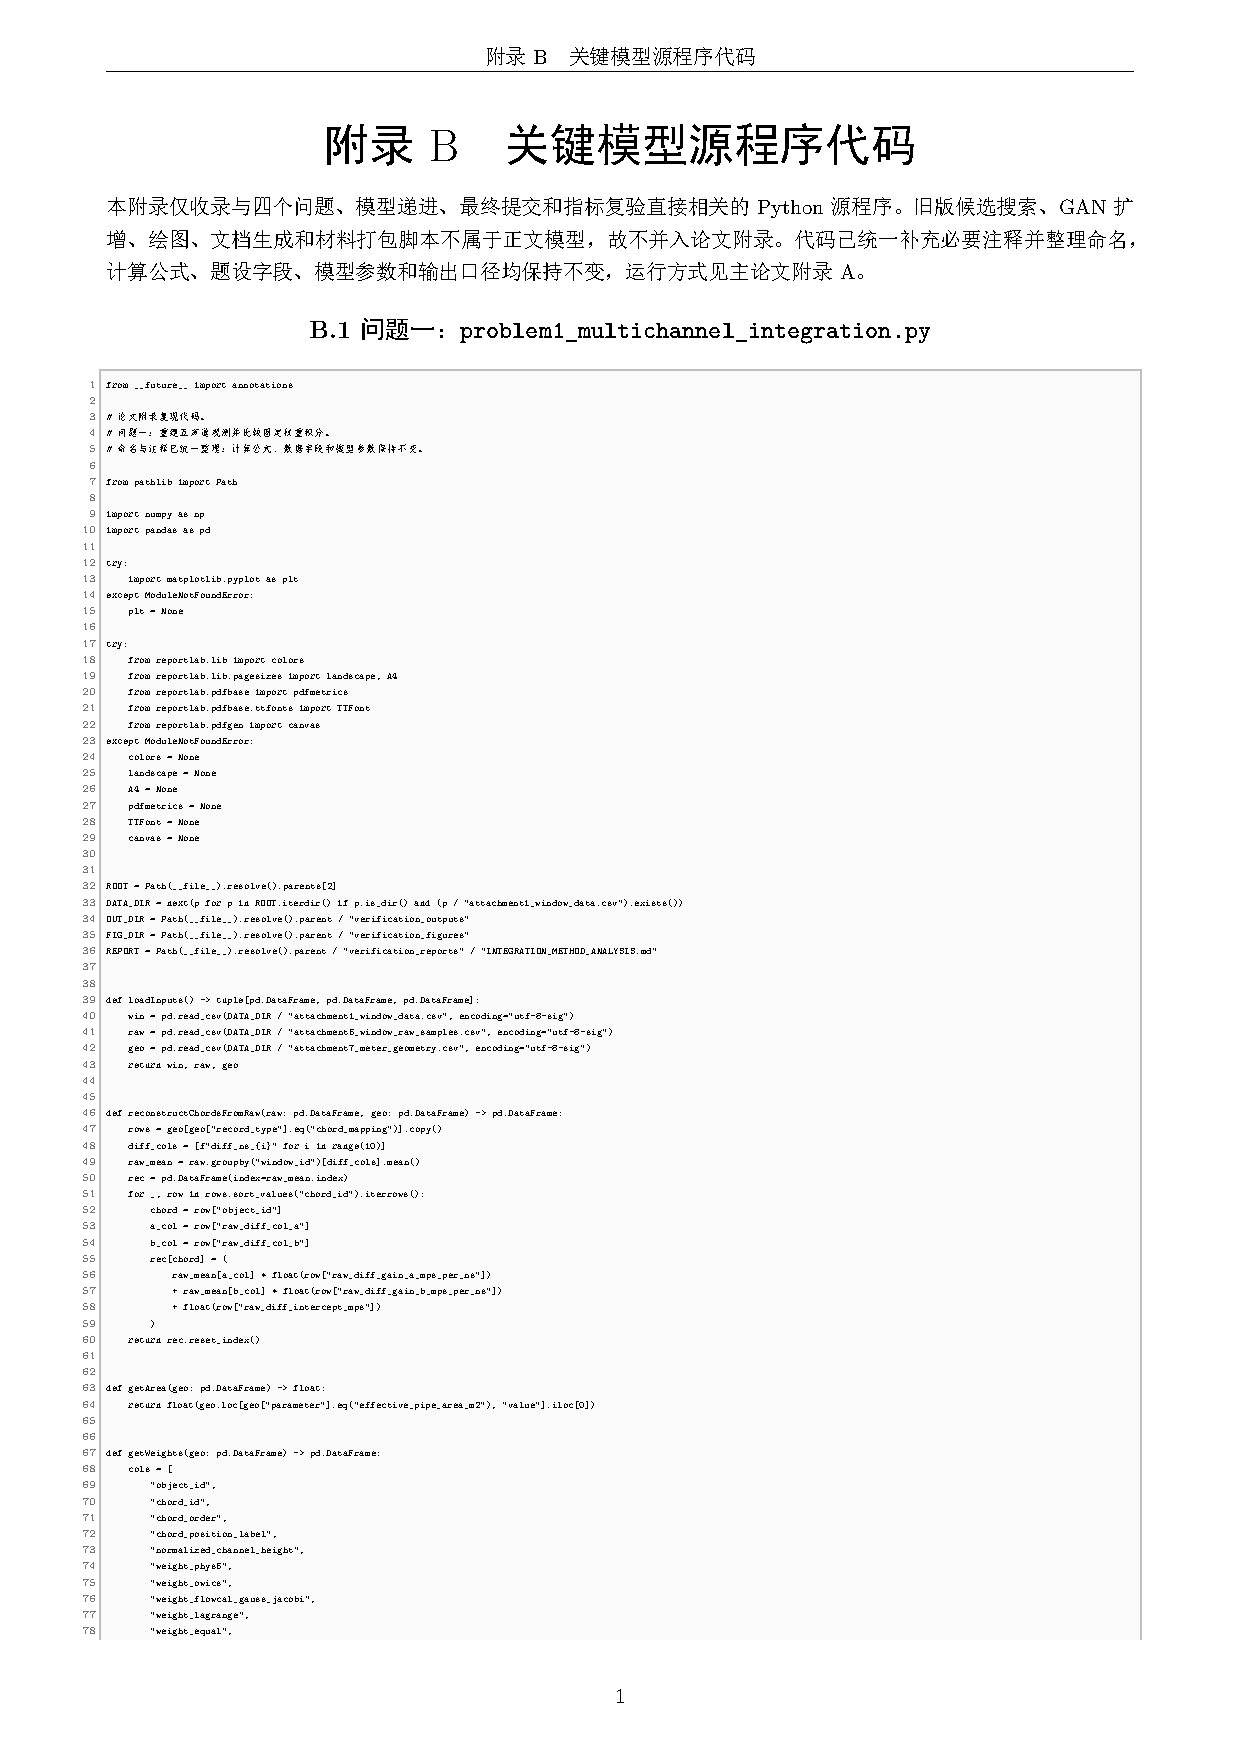
\includepdf[pages=-]{附录B_完整源程序代码.pdf}%
}

\newcommand{\threelinetable}[4]{%
  \begin{center}
    {\fontsize{10.5pt}{12.6pt}\heiti\bfseries #1}\par
    \vspace{0.6em}
    \begin{tabular}{#2}
      \toprule
      #3 \\
      \midrule
      #4 \\
      \bottomrule
    \end{tabular}
  \end{center}
}

\begin{document}

\vspace*{0.55cm}
\papertitle{扰流条件下超声波流量计的多声道补偿建模}

\vspace{0.35cm}

\abstractcn{%
超声波流量计利用顺流和逆流的声传播时间并不相同这一差异求取轴向流速。然而现实条件下各种因素产生的扰流会使圆管速度剖面偏斜，并改变各声道对截面平均速度的代表性。本文以多声道物理积分为主尺度，结合无扰流标定、剖面特征和受约束核回归，完成四个问题的建模与检验。

针对问题一，先由顺流、逆流传播时间建立单声道速度与窗口体积公式，再说明单条声道无法完整代表非均匀截面速度。再依据附件中的声道位置、等效面积和固定权重构造五声道积分，在统一口径下比较 Phys6、Lagrange、OWICS 与等权积分，最后选取表现最优秀的 Phys6 作为后续建模的物理基线。

针对问题二，从附件中筛选无扰流参考窗口，以 Phys6 为初始估计，构造仅随流量规模变化的二次校准曲线。曲线参数只用训练部分估计，并通过不同流量点的相对误差、组均值与重复性比较，判断正常工况校准能够修正的误差范围。

针对问题三，从五声道响应中提取流量尺度、径向剖面差、A/B 方向不对称、旋流代理以及少量动态与零点稳定性特征，再结合效应量、单特征 AUC、PCA 和多种聚类方法检验特征作用及扰流状态的可分性。最终结果表明，多数扰流状态在在线特征空间中连续重叠。

针对问题四，以固定物理积分为起点，依次用 Ridge 检验线性补偿能力，用 ANN 验证非线性残差学习的适用性，再以紧凑物理特征建立 RBF-KRR。随后引入逐秒稳定性信息构造多核 KRR，并在固定模型结构后加入受约束的无扰流后校准。标签盲验证用于检验未参与训练窗口，最终全量标定结果则只用于题目给定窗口的体积输出，两种口径分别报告。%
}{%
超声波流量计；多声道积分；扰流补偿；RBF 核岭回归；剖面可分性%
}

\section{问题重述与分析}

\subsection{问题背景}

顺流和逆流的声传播时间并不相同，超声波流量计正是利用这一差异求取轴向流速。对流速作时间与截面积分，就可以得到窗口体积。单声道在理想剖面下能够给出有效估计，实际管路却很少保持在理想状态。弯头、阀门、缩径段或其他扰流件会改变速度分布，偏流与旋流也随之出现。

已有工作从不同角度处理这一误差。Mousavi 等借助半三维仿真求取几何剖面修正因子；Sakhavi 和 Nouri 用广义速度剖面降低积分结果对流场偏离的敏感程度。Papathanasiou 等关注声道布置与扰流修正的配合，Zhao 等则用 ANN 融合多路径观测\cite{Mousavi2020FPCF,Sakhavi2022GeneralizedProfile,Papathanasiou2022FlowDC,Zhao2014ANN}。这些研究为本文提供了一个清晰起点：物理积分负责确定流量主尺度，剖面特征与受约束补偿用于处理偏差。

本题给出一台五声道超声波流量计的窗口化测试数据，包含标准体积、基础积分估计量、五条等效声道观测量、A/B 方向差异、剖面特征、启停动态特征和零点状态特征。建模目标是在不使用标准体积、日期、窗口编号等非运行时信息作为在线输入的前提下，输出每个窗口的估计体积，并在无扰流线性度、重复性和扰流综合指标上达标。

\subsection{数据概况}

主数据表记录了 $159$ 个窗口，每个窗口包含 $40$ 个字段。D0 无扰流参考样本只有 $10$ 个；其余 $149$ 个窗口来自 D1 至 D8 八种扰流条件。数据覆盖的名义流量点为 20、30、40、50、60、70 和 80。题目评价脚本计算部分指标时采用 40 至 100 的有效范围。

窗口内原始观测序列共有 $29322$ 行，能够通过窗口编号回接主表。另一个几何参数表给出了等效半径、截面积、五条声道的位置与映射关系，同时提供多套固定积分权重。

泛化评价采用三层验证。首先，以日期、流量点和扰流编号构成分层单元，形成 $118$ 个训练窗口与 $41$ 个验证窗口的标签盲示例划分；其次，固定模型配置，在 $40$ 个不同随机种子的同类分层划分上统计性能波动；最后，将完整分层单元留作验证，实施整组留出压力测试。划分过程只利用样本的分组信息，不查看标准体积。模型应用于新日期时，应预先固定特征、核参数和校准形式，并使用独立数据检验。

\subsection{问题拆解}

问题一要求从传播时间差模型推导单声道体积估计公式，并解释多声道积分权重的物理含义；问题二要求在无扰流数据上建立多声道标定模型，并通过相对误差、组均值误差和组内重复性评价其稳定性；问题三要求分析扰流下的剖面、A/B 差异、动态和零点特征，构造不依赖人工扰流编号的在线识别与补偿方法；问题四要求整合前三问，形成固定规则和参数的最终窗口体积估计模型，并用题目给定评价脚本输出窗口误差、组达标数和三项综合指标。

\section{模型假设}

（1）几何与声道参数假设。题目给出的等效管道半径、截面积、声道长度、声道位置及固定积分权重均视为测试前已知常数；五条等效声道观测量分别表征不同截面高度的平均流速贡献。

（2）数据使用假设。标准体积只作为训练标签和评价基准；日期、窗口编号及人工扰流编号仅用于离线分组、验证和机理解释，不进入在线预测。对相近流量与剖面状态，短时间内的主要误差可由剖面、动态和零点特征描述。

（3）模型复杂度假设。样本数量有限，候选补偿器采用参数规模受控的线性方法或带正则化的核方法；高维模型仅用于检验样本内表达能力，不将偶然结构解释为未知工况上的稳定规律。

\section{符号说明}

\begin{longtable}{cl}
\toprule
符号 & 含义 \\
\midrule
\endfirsthead
\toprule
符号 & 含义 \\
\midrule
\endhead
$L$ & 声道长度 \\
$\theta$ & 声道与管道轴线夹角 \\
$t_+$, $t_-$ & 顺流、逆流传播时间 \\
$v$ & 管道轴向平均流速 \\
$A$ & 等效管道截面积 \\
$T_i$ & 第 $i$ 个窗口持续时间 \\
$V_i^{\mathrm{std}}$ & 第 $i$ 个窗口标准体积 \\
$\hat V_i$ & 第 $i$ 个窗口模型估计体积 \\
$c_{ij}$ & 第 $i$ 个窗口第 $j$ 条等效声道观测量 \\
$w_j$ & 第 $j$ 条声道积分权重 \\
$e_i$ & 第 $i$ 个窗口相对误差 \\
$g$ & 官方评价组，$g=(\mathrm{date},\mathrm{flow\ point})$ \\
$h$ & 训练分层和压力测试单元，$h=(\mathrm{date},\mathrm{flow\ point},\mathrm{disturbance\ id})$ \\
$Dk,q$ & 扰流综合指标中的扰流编号--流量点集合 \\
$\bar e_g$ & 评价组 $g$ 的平均相对误差 \\
$SD_g$ & 评价组 $g$ 的组内重复性标准差 \\
$u_{\mathrm{nor},L}$ & 无扰流线性度等效量 \\
$u_{\mathrm{nor},r}$ & 重复性等效量 \\
$u_{\mathrm{nor},d}$ & 扰流综合不确定度等效量 \\
\bottomrule
\end{longtable}

\section{问题一：基础传播模型与多声道积分}

\subsection{单声道测量原理解释}

设声波沿长度为 $L$、与管道轴线夹角为 $\theta$ 的声道传播，流体声速为 $c$，管道轴向平均流速为 $v$。顺流和逆流传播时间可表示为
\begin{equation}
t_+ = \frac{L}{c + v\cos\theta}, \qquad
t_- = \frac{L}{c - v\cos\theta}.
\end{equation}
两式相减并整理，可得声道方向上的流速估计：
\begin{equation}
v = \frac{L}{2\cos\theta}\left(\frac{1}{t_+}-\frac{1}{t_-}\right).
\label{eq:single_velocity}
\end{equation}
若第 $i$ 个窗口持续时间为 $T_i$，等效管道截面积为 $A$，则单声道窗口体积估计为
\begin{equation}
\hat V_i = A T_i v_i.
\label{eq:single_volume}
\end{equation}
该模型结构清晰，参数物理含义明确，但它只代表单条声道上的线平均速度信息，而体积流量取决于整个圆截面的速度积分\cite{Sakhavi2022GeneralizedProfile}。因此，当截面速度剖面不均匀时，单声道速度未必等于截面平均速度。

\subsection{五声道加权积分与基础方法比较}

一条声道只覆盖截面的局部信息。为了接近截面真实平均流速，需要把不同高度处的观测按照其代表区域进行组合。声道位置、剖面识别方式以及积分权重都会影响最终的重构精度\cite{Qin2016ProfileIdentification,XiangMultipathIntegration}。还有论文提出广义速度剖面或修正因子降低固定权重对特定流型的依赖\cite{Sakhavi2022GeneralizedProfile,Gryshanova2023CorrectionFactor}。对窗口 $i$，记五条等效声道观测为 $c_{i0},\ldots,c_{i4}$，相应权重为 $w_0,\ldots,w_4$，则平均速度代理量写成
\begin{equation}
\bar v_i = \sum_{j=0}^{4} w_j c_{ij},
\end{equation}
窗口体积估计为
\begin{equation}
\hat V_i = A T_i \bar v_i.
\end{equation}
声道权重反映了各声道所代表的截面区域面积贡献或数值积分节点权重。中心声道通常对中心区域速度贡献更敏感，边缘声道可补充靠近管壁区域的速度信息。

需要说明的是，附件中的 \texttt{chord0}--\texttt{chord4} 已经由题设声道映射整理为等效声道观测量。本文在式中将 $c_{ij}$ 作为等效速度观测使用；若直接从原始传播时间或原始声道量计算，则还需通过附件给出的映射和几何系数先换算为同一量纲的等效速度代理。

附件给出的五声道位置和固定权重见表~\ref{tab:integration_weights}。Phys6 是题设提供的工程积分基线；OWICS 与 Gauss-Jacobi 在附件中的权重数值一致，统计时合并为一组先验。Lagrange 通过插值重构剖面后再积分，因而提高了两侧边缘声道的权重。等权法不区分声道代表面积和截面位置，在非均匀剖面下通常误差较大。

\begin{table}[H]
\centering
\caption{五声道位置与固定积分权重}
\label{tab:integration_weights}
\small
\begin{tabular}{lccccc}
\toprule
声道 & 归一化高度 & Phys6 & OWICS & Lagrange & 等权 \\
\midrule
chord0 & 0.7274 & 0.209874 & 0.221205 & 0.266260 & 0.200000 \\
chord1 & 0.2662 & 0.153223 & 0.112176 & 0.096121 & 0.200000 \\
chord2 & 0.0000 & 0.266827 & 0.333238 & 0.275238 & 0.200000 \\
chord3 & -0.2662 & 0.153223 & 0.112176 & 0.096121 & 0.200000 \\
chord4 & -0.7274 & 0.209874 & 0.221205 & 0.266260 & 0.200000 \\
\bottomrule
\end{tabular}
\end{table}

表~\ref{tab:baseline_mae} 汇总了四种基础积分量的窗口误差。Phys6 与 Lagrange 的 MAE 很接近，均明显低于 OWICS 和等权积分。两者的优势并不完全相同：Lagrange 的平均偏差更接近零，Phys6 则具有较小的最大绝对误差。因此，后续补偿实验将 Phys6 与 Lagrange 保留为候选物理基准。基础积分方法的比较如图~\ref{fig:mae_compare} 所示。

\begin{table}[H]
\centering
\caption{基础积分方法窗口误差比较}
\label{tab:baseline_mae}
\begin{tabular}{lccc}
\toprule
方法 & MAE(\%) & ME(\%) & 最大绝对误差(\%) \\
\midrule
Phys6 & 0.180653 & -0.136424 & 0.495146 \\
OWICS & 0.506237 & 0.506237 & 1.000727 \\
Lagrange & 0.183613 & -0.007930 & 0.644012 \\
Equal Weight & 0.637292 & 0.637292 & 1.083603 \\
\bottomrule
\end{tabular}
\end{table}

\begin{figure}[!htbp]
  \centering
  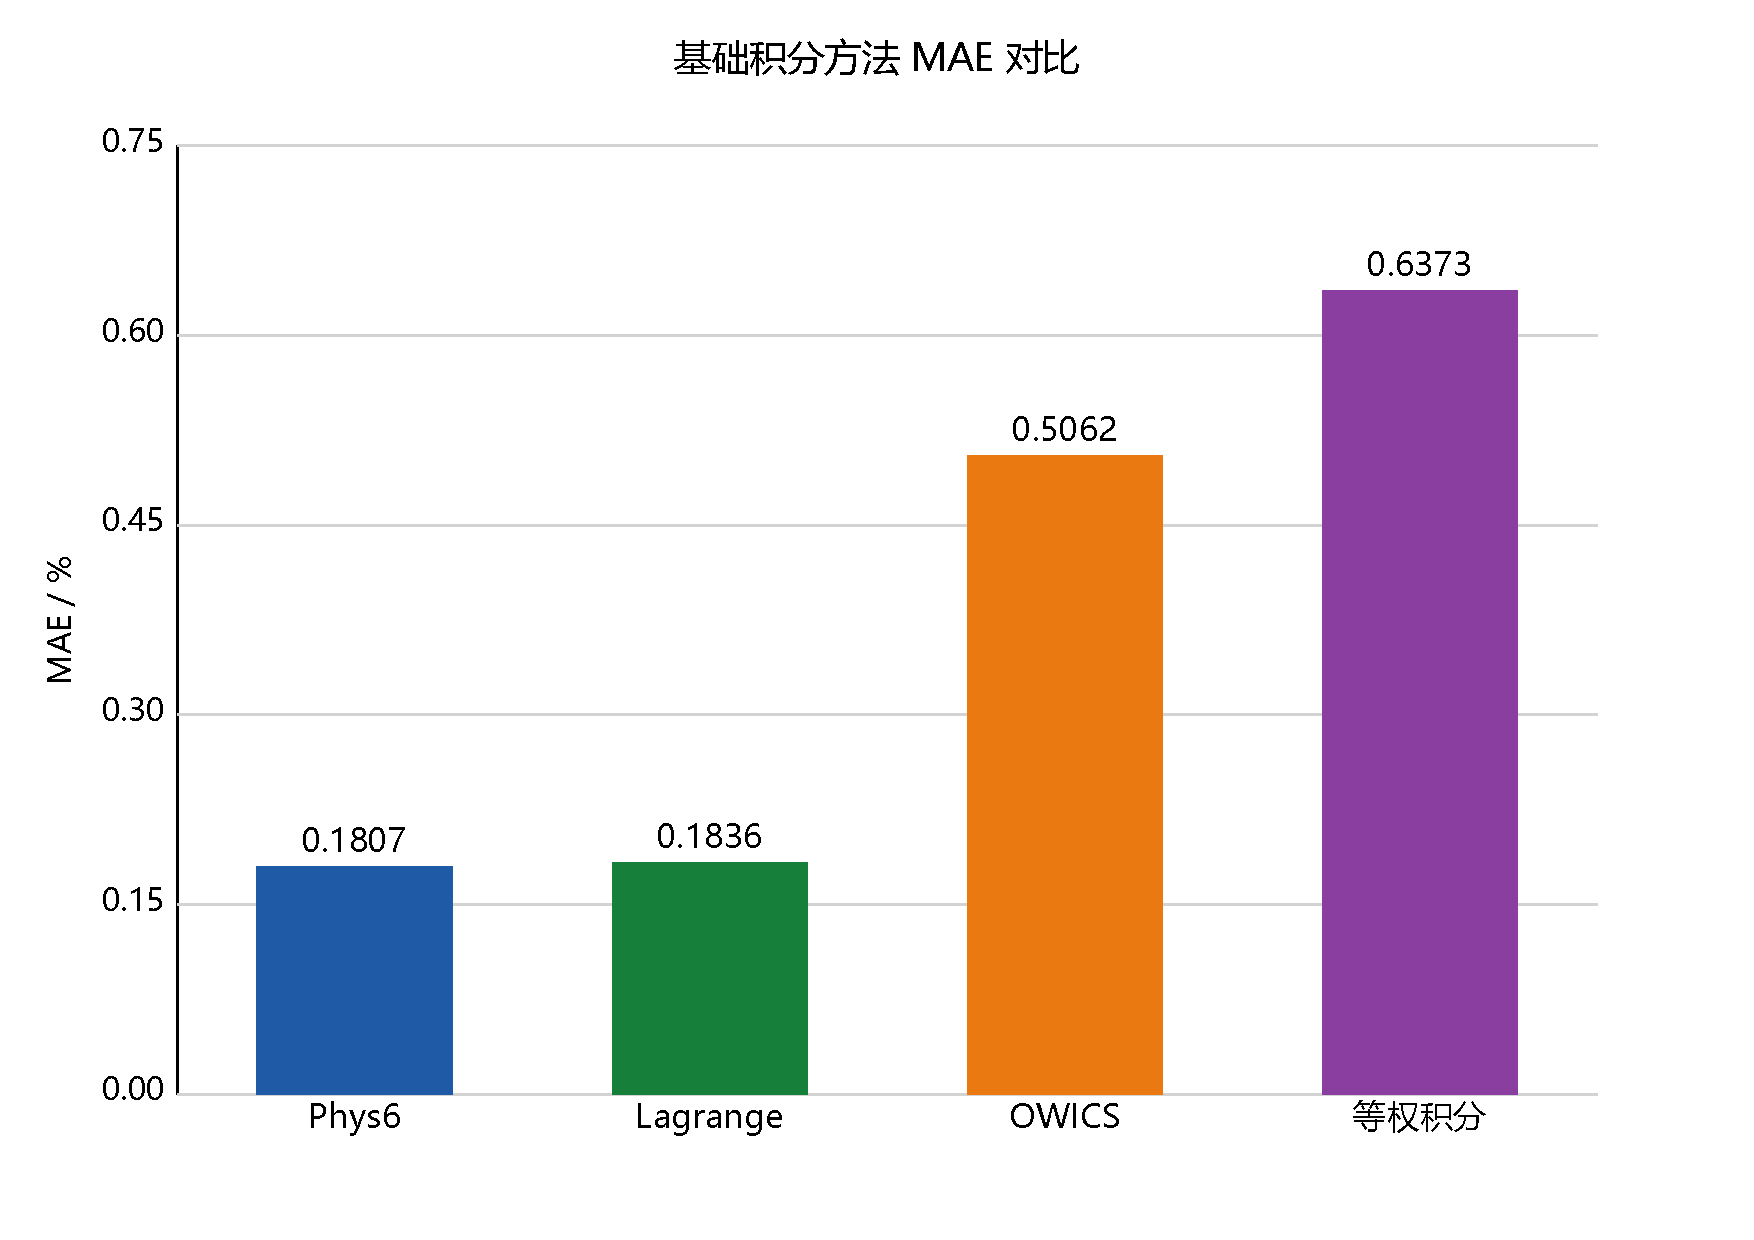
\includegraphics[width=0.88\textwidth]{../figures/fig_model_mae_comparison.pdf}
  \caption{基础积分方法 MAE 对比}
  \label{fig:mae_compare}
\end{figure}

进一步按流量点观察，如图~\ref{fig:integration_flow_mae} 所示，Phys6 和 Lagrange 在多数流量点上保持较低 MAE，而 OWICS 与等权法在部分流量段误差明显放大。这说明固定权重积分虽然能提供稳定的物理主尺度，但仍会随流量点和剖面形态发生系统偏差。

\begin{figure}[!htbp]
  \centering
  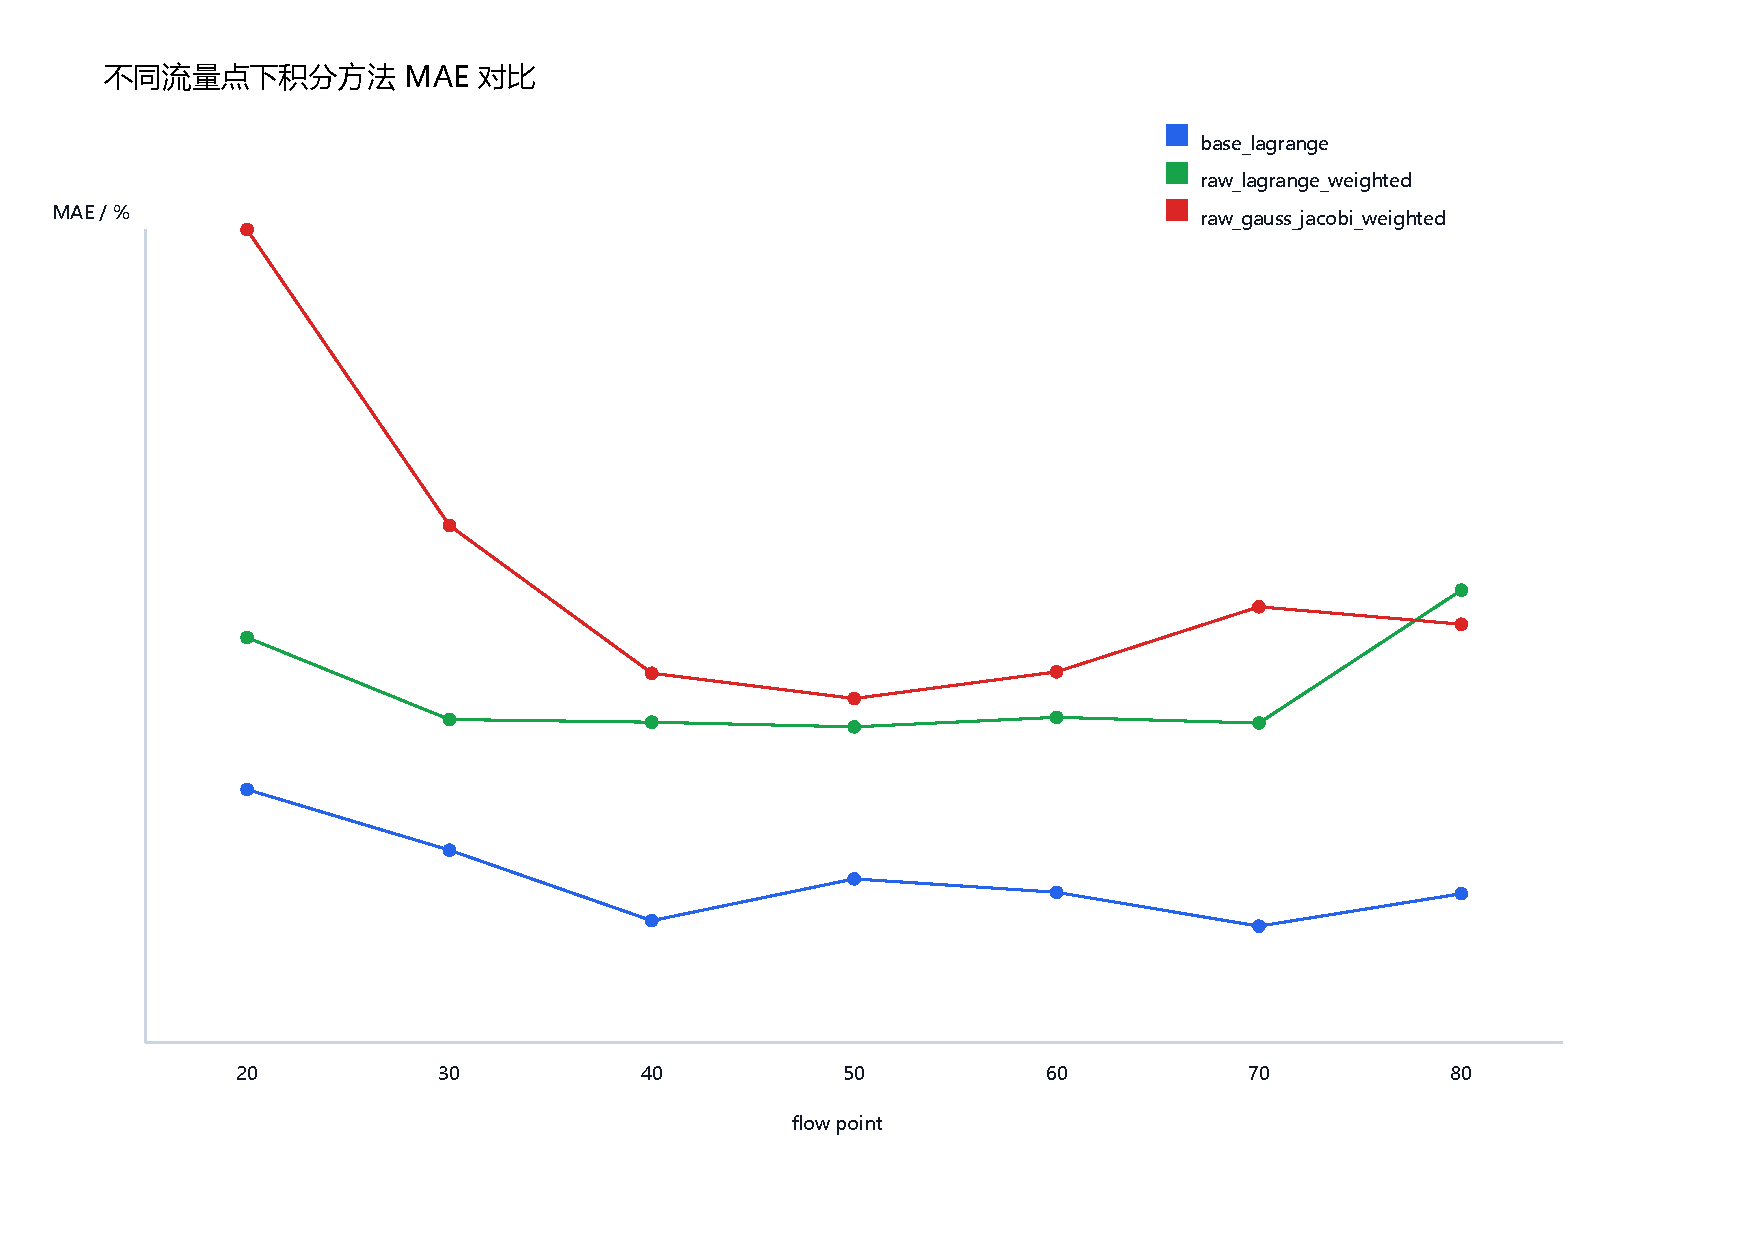
\includegraphics[width=0.88\textwidth]{../figures/fig_integration_flow_mae.pdf}
  \caption{不同流量点下基础积分方法 MAE 对比}
  \label{fig:integration_flow_mae}
\end{figure}

按工况拆分后，四种方法的表现见表~\ref{tab:baseline_condition_mae}。OWICS/Gauss--Jacobi 先验在 D0 正常工况下最优，但在 D1--D8 扰流下误差明显增加；Phys6 和 Lagrange 在扰流样本上更稳定。这说明固定积分权重与其假设的速度剖面有关，正常剖面上的最优权重不一定适合畸变剖面。

\begin{table}[H]
\centering
\caption{基础积分方法在不同工况下的 MAE（\%）}
\label{tab:baseline_condition_mae}
\begin{tabular}{lcc}
\toprule
方法 & D0 无扰流 & D1--D8 扰流 \\
\midrule
Phys6 & 0.388727 & 0.166688 \\
Lagrange & 0.523550 & 0.160799 \\
OWICS/Gauss--Jacobi & 0.226394 & 0.525019 \\
Equal Weight & 0.414760 & 0.652227 \\
\bottomrule
\end{tabular}
\end{table}

\section{问题二：无扰流正常工况校准}

\subsection{问题分析}

附件中标记为无扰流参考工况的窗口反映了仪表在正常速度剖面下随流量变化的固有偏差。因此，该部分数据可以作为正常工况校准依据。

\subsection{问题建模}

令问题一中选定的 Phys6 工程积分估计量为
\begin{equation}
V_{b,i}=V_{\mathrm{Phys6},i}.
\end{equation}
在无扰流状态下，可引入只依赖流量规模的百分数正常校准曲线 $c_0^{(\%)}(q)$，得到
\begin{equation}
V_{N,i}=V_{b,i}\left[1+\frac{c_0^{(\%)}(q_i)}{100}\right],
\label{eq:d0_curve}
\end{equation}
其中 $q_i$ 为归一化流量点。程序中采用的归一化公式为
\begin{equation}
q_i=\frac{\mathrm{flow\ point}_i-50}{30}.
\end{equation}
本文采用二次平滑形式
\begin{equation}
c_0^{(\%)}(q)=b_0+b_1q+b_2q^2,
\end{equation}
并在 D0 窗口上用带岭惩罚的最小二乘估计参数，以避免少量无扰流样本造成过拟合。

这里的 $q_i$ 取题目提供的名义流量点并归一化，表示运行时流量规模，不读取标准装置体积。

在标签盲示例划分中，训练集含有 $7$ 个 D0 窗口。表中系数只由这些训练窗口估计，$41$ 个验证窗口不参与参数求解。结果见表~\ref{tab:d0_curve_coef}。这里的曲线直接修正 Phys6 基线，与问题四在 KRR 之后拟合的 D0 残余后校准曲线不同。

\begin{table}[H]
\centering
\caption{标签盲示例划分训练集上的 Phys6 无扰流校准曲线系数}
\label{tab:d0_curve_coef}
\begin{tabular}{lcc}
\toprule
项 & 系数(\%) & 曲线形式 \\
\midrule
$b_0$ & 0.402727 & $c_0^{(\%)}(q)=b_0+b_1q+b_2q^2$ \\
$b_1$ & -0.033031 & 同上 \\
$b_2$ & -0.007535 & 同上 \\
\bottomrule
\end{tabular}
\end{table}

\subsection{结果分析}

无扰流校准曲线只描述正常流态中随流量变化的系统偏差，不能表达弯管、旋流或非充分发展流造成的附加剖面畸变。因此，本节重点考察正常工况线性度与流量点残差，不能把该曲线直接视为扰流补偿模型。

在标签盲示例划分消融中，仅使用 Phys6 时
\begin{equation}
u_{\mathrm{nor},L}=0.462931\% .
\end{equation}
加入 D0 曲线后，
\begin{equation}
u_{\mathrm{nor},L}=0.055310\% ,
\end{equation}
说明正常流量点系统偏差被显著削弱。但同一消融中，
\begin{equation}
\mathrm{MAE}:0.179991\%\rightarrow 0.260279\%,
\qquad
u_{\mathrm{nor},d}:0.217668\%\rightarrow 0.218491\%,
\end{equation}
没有同步改善。这说明无扰流曲线能够削弱正常流量点的系统偏差，但不能代表扰流状态下的补偿效果。

无扰流内部实验还表明，带对称权重约束的 OWICS/Gauss-Jacobi 先验与剖面修正模型在正常窗口上误差较低；但直接作用于其余扰流窗口后，误差明显增大。因此，正常工况下得到的最优积分或校准关系不能直接外推到畸变剖面。

综上，问题二得到一条只描述正常工况流量相关偏差的校准曲线，为下一步分析扰流造成的额外剖面变化提供了一个基准。

从 D0 内部逐流量点结果看，校准模型在 $40,50,60,70,80$ 五个流量点的 MAE 分别为 $0.046174\%$、$0.035041\%$、$0.027378\%$、$0.057486\%$ 和 $0.036046\%$。其中 $70$ 流量点残余误差最大，仍需更多正常锚点；$40$ 流量点仅有一个窗口，不能据此判断重复性。由于 D0 全部来自同一天，上述结果属于正常工况内部拟合分析，而不是跨日期验证。

\section{问题三：扰流机理识别与聚类可分性分析}

\subsection{扰流特征构造与重要性分析}

扰流状态会改变圆管截面速度剖面，使不同声道对截面平均速度的代表性发生变化。Zhao 等的 CFD 研究表明，双弯管等复杂管路可产生强非对称与旋流剖面，声道方向会影响多路径流量计的积分误差；Papathanasiou 等进一步通过流动仿真说明，扰流入口条件下的声道布置和修正因子需要协同设计\cite{Zhao2014CFD,Papathanasiou2022FlowDC}。国内关于上游扰流和非充分发展流的研究也观察到扰流条件对计量准确度及不同声道响应的显著影响\cite{JinUpstreamDisturbance,SuUnderdevelopedFlow}。

Sakhavi 和 Nouri 的广义速度剖面研究说明，固定积分规则的精度依赖其假设的速度分布；当实际剖面偏离该假设时，需要利用多声道状态降低模型敏感性\cite{Sakhavi2022GeneralizedProfile}。剖面修正因子与在用误差补偿研究通常保留物理估计的主尺度，再对稳定系统残差进行标定\cite{Mousavi2020FPCF,Gryshanova2023CorrectionFactor,Li2023MLInUse}；这一思路为从多声道剖面特征解释扰流附加误差提供了依据。据此，本文构造自定义紧凑物理特征集（compact physical features）描述在线剖面状态，没有把人工扰流编号 \texttt{disturbance\_id} 作为模型输入。

为直观说明上述机理，图~\ref{fig:disturbance_profile_representativeness} 按附件 7 给定的五声道位置绘制剖面示意，并列出附件 1 中同一流量点下 D0 与 D3 窗口均值的代表性对比。彩色云图用于说明速度剖面由近似对称向偏斜状态变化。

\begin{figure}[!htbp]
  \centering
  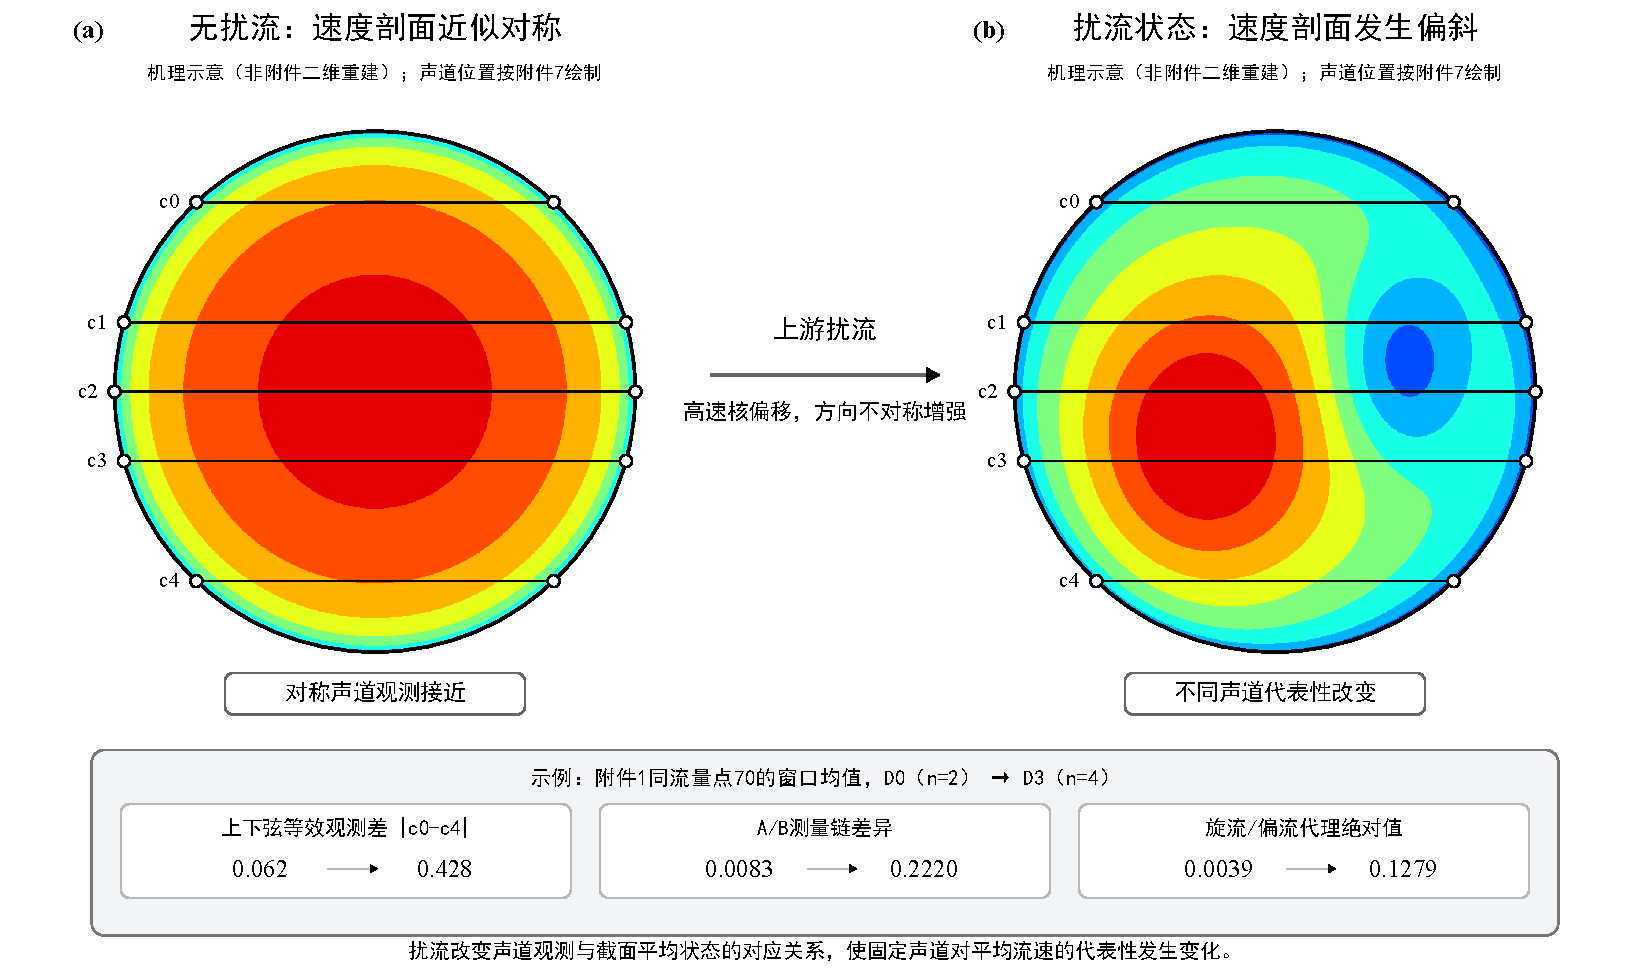
\includegraphics[width=0.98\textwidth]{../figures/fig_disturbance_profile_representativeness.pdf}
  \caption{扰流导致速度剖面偏斜及声道代表性变化示意}
  \label{fig:disturbance_profile_representativeness}
\end{figure}

流量尺度由 $q$ 和 $q^2$ 表示。剖面形态不再用单个声道概括，而是考察中心相对整体的偏离、边缘与内侧差异以及上下响应差。A/B 方向不对称和旋流分别由 \texttt{profile\_ab\_abs}、\texttt{profile\_swirl} 等变量描述。动态与零点变量只保留少量稳定性指标，主要用于追踪重复性失稳。

不同积分规则的分歧还提供了另一条线索。本文定义
\begin{equation}
\Delta_{\mathrm{Lag-Phys6},i}
=\frac{V_{\mathrm{Lag},i}-V_{\mathrm{Phys6},i}}{V_{\mathrm{Phys6},i}}.
\end{equation}
正常剖面下，两种积分结果通常相近。剖面发生畸变后，权重对各声道响应的差异会被放大，$\Delta_{\mathrm{Lag-Phys6},i}$ 也一般会随之变化。虽然它不是直接测得的流场量，但可以作为剖面偏离程度的间接指标。

为判断哪些在线变量能够用于识别扰流，我们综合使用标准化效应量、单特征 AUC、L2 Logistic 标准化系数和置换重要性。对第 $j$ 个特征，D0 与扰流窗口的标准化效应量定义为
\begin{equation}
d_j=\frac{|\mu_{D,j}-\mu_{0,j}|}{s_{\mathrm{pooled},j}},
\end{equation}
其中 $\mu_{D,j}$ 和 $\mu_{0,j}$ 分别为扰流窗口和 D0 窗口上的均值，合并标准差为
\begin{equation}
s_{\mathrm{pooled},j}
=\sqrt{\frac{(n_D-1)s_{D,j}^2+(n_0-1)s_{0,j}^2}{n_D+n_0-2}}.
\end{equation}

表~\ref{tab:disturbance_feature_importance} 给出综合排序靠前的特征。可以看到，\texttt{profile\_swirl} 和 \texttt{profile\_ab\_abs} 的效应量分别达到 $45.7715$ 和 $32.8618$，单特征 AUC 均为 $1.0000$。这说明区分无扰流与扰流状态最有效的变量主要来自旋流代理、A/B 方向不对称和径向剖面变化，而不是单纯的流量规模变量。

\begin{table}[H]
\centering
\caption{扰流识别特征重要性前 8 项}
\label{tab:disturbance_feature_importance}
\scriptsize
\begin{tabular}{p{0.40\textwidth}cccc}
\toprule
特征 & 效应量 & AUC & Logistic 系数绝对值 & 置换损失增量 \\
\midrule
\texttt{profile\_swirl} & 45.7715 & 1.0000 & 0.4491 & 0.04237 \\
\texttt{profile\_ab\_abs} & 32.8618 & 1.0000 & 0.4479 & 0.04123 \\
\texttt{ab\_abs\_mean} & 2.4865 & 1.0000 & 0.2182 & 0.00655 \\
\texttt{lagrange\_volume\_m3\_minus}\newline\texttt{phys6\_frac} & 2.3402 & 0.9785 & 0.1432 & 0.00262 \\
\texttt{chord\_edge\_minus}\newline\texttt{inner\_frac} & 2.3372 & 0.9785 & 0.1430 & 0.00271 \\
\texttt{profile\_edge\_inner} & 2.3239 & 0.9785 & 0.1420 & 0.00279 \\
\texttt{owics\_volume\_m3\_minus}\newline\texttt{phys6\_frac} & 2.0918 & 0.9906 & 0.1416 & 0.00271 \\
\texttt{zero\_rate\_med} & 1.4052 & 1.0000 & 0.1374 & 0.00222 \\
\bottomrule
\end{tabular}
\end{table}

\begin{figure}[!htbp]
  \centering
  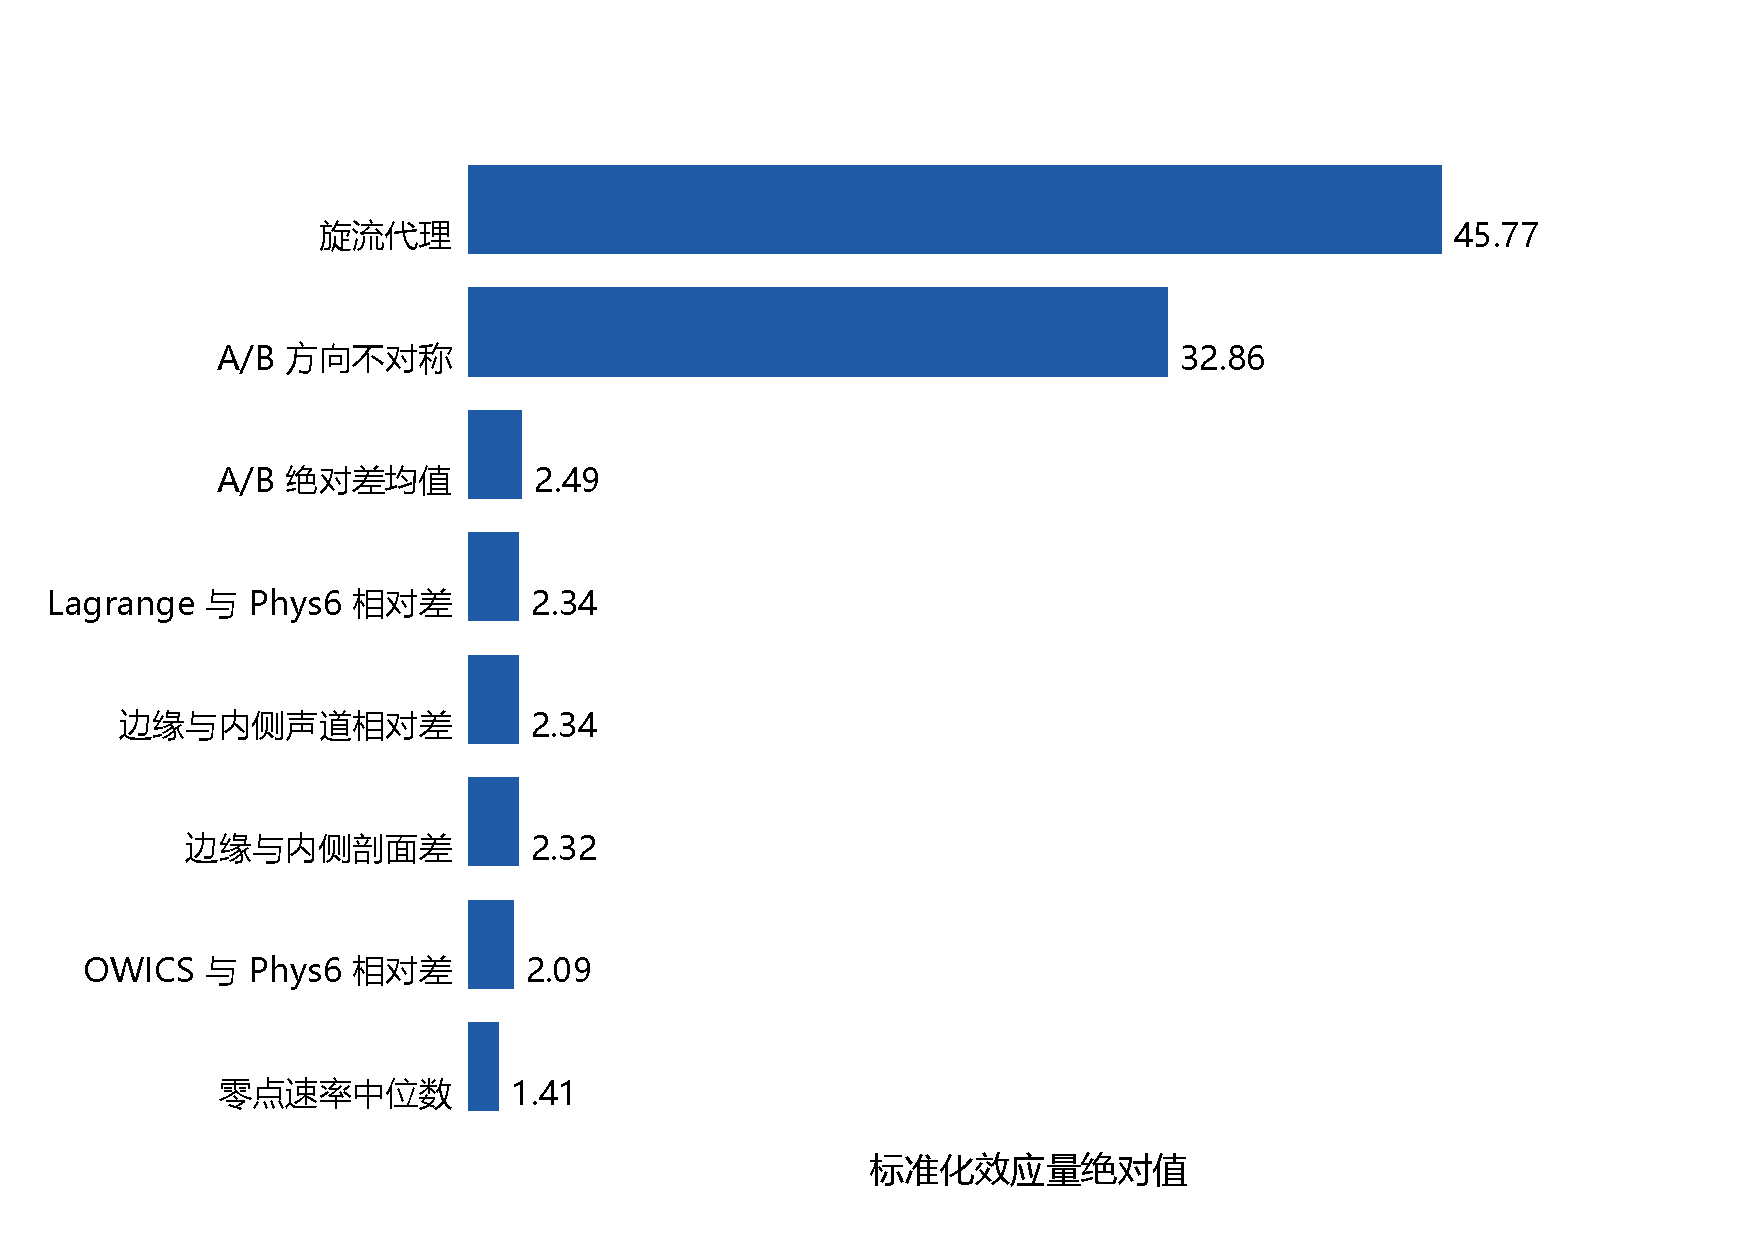
\includegraphics[width=0.88\textwidth]{../figures/fig_disturbance_feature_importance.pdf}
  \caption{扰流识别特征效应量排序}
  \label{fig:disturbance_feature_importance}
\end{figure}

\subsection{降维、聚类与失效机制}

PCA 只在 D1 至 D8 的扰流窗口上实施，输入为标准化后的紧凑物理特征。PC1 和 PC2 分别解释 $39.7544\%$ 与 $22.0094\%$ 的方差，二维累计解释率为 $61.7638\%$。加入第三个主成分后，该比例升至 $76.1964\%$；前五个主成分可覆盖 $90.1991\%$。

主要变化可以被少量主成分压缩，但二维图仍会丢失接近四成的信息。因此，图中的重叠不能简单解释成工况完全相同，分离现象也视高维结果综合判断。

\begin{figure}[!htbp]
  \centering
  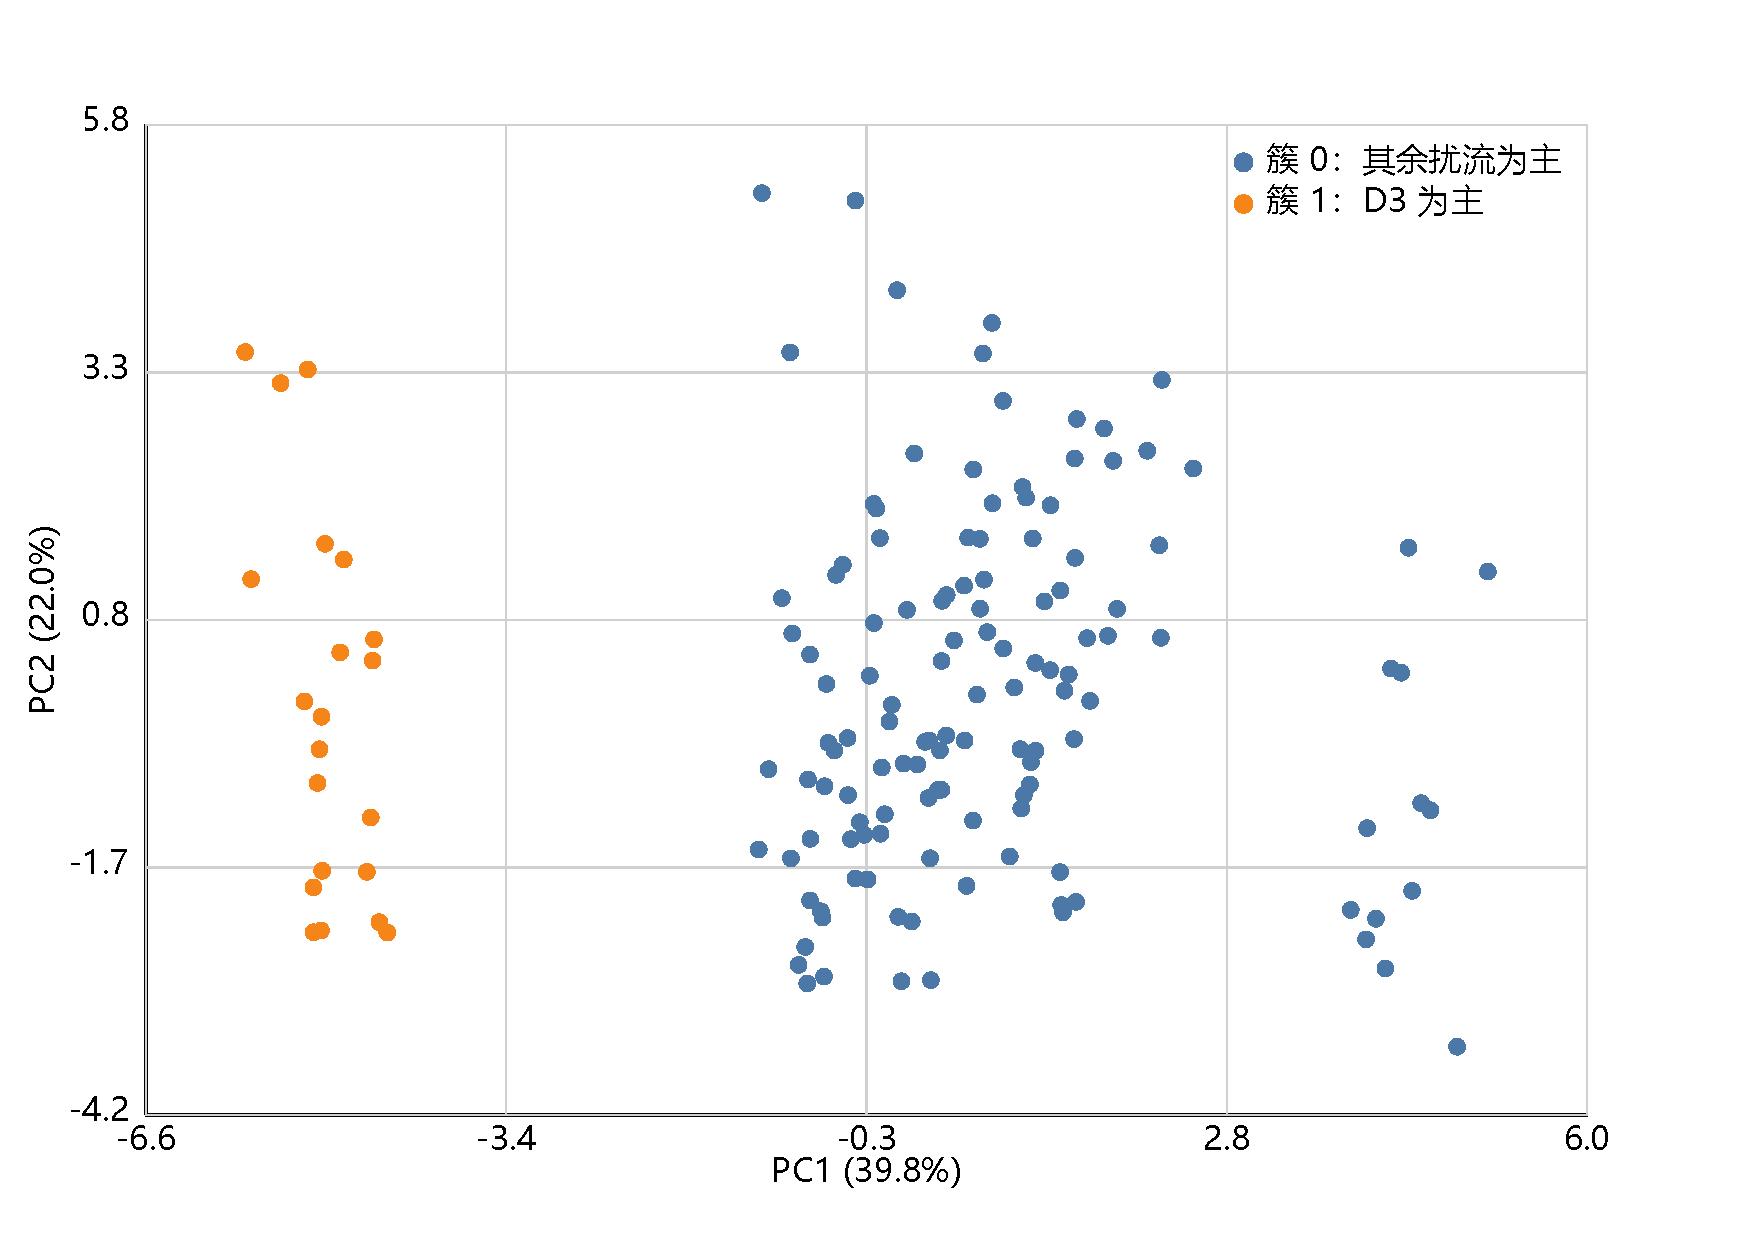
\includegraphics[width=0.86\textwidth]{../figures/fig_disturbance_pca_clusters.pdf}
  \caption{D1 至 D8 扰流窗口的 PCA 投影与最佳聚类}
  \label{fig:disturbance_pca}
\end{figure}

Qin 等曾用多声道观测训练 SVM，对 $65$ 种预设流型进行分类\cite{Qin2016ProfileIdentification}。说明多声道信息具备识别流型的潜力，但前提是类别边界清楚，训练样本也有足够覆盖。

本文分别运行 KMeans、Ward 层次聚类和对角 GMM，考察 $K=2,\ldots,5$。候选结果由 Silhouette、Calinski--Harabasz 与 Davies--Bouldin 指标共同评价。$K=2$ 的 KMeans 与 Ward 得到相同划分，三项指标均并列最优，分别为 $0.377676$、$56.9208$ 和 $0.98888$。后文采用 KMeans 标签展示交叉表。该轮廓系数只显示中等结构，并不支持强可分结论。

表~\ref{tab:cluster_disturbance_cross} 给出最佳聚类与人工扰流编号的交叉表。可以看到，一个簇几乎完全对应 D3，而 D1、D2、D4、D5、D6、D7、D8 大规模重叠在另一个簇中。这说明 \texttt{disturbance\_id} 更适合作为离线实验条件标签，而不能直接看作是在线流型类别。

\begin{table}[H]
\centering
\caption{最佳聚类与扰流编号交叉表}
\label{tab:cluster_disturbance_cross}
\begin{tabular}{ccccccccc}
\toprule
Cluster & D1 & D2 & D3 & D4 & D5 & D6 & D7 & D8 \\
\midrule
0 & 21 & 23 & 0 & 22 & 17 & 14 & 13 & 18 \\
1 & 0 & 0 & 21 & 0 & 0 & 0 & 0 & 0 \\
\bottomrule
\end{tabular}
\end{table}

把聚类标签与整组留出的失效诊断放在一起后，结论更为直接。系统漂移样本与重复性失稳样本混在同一簇中。D3 的位置相对独立，其他扰流编号却没有形成对应边界。若此时先做硬分类，再为每个簇训练独立补偿器，前一级的错分会继续传入流量估计。但是现有数据不足以支撑这条路线。

聚类未形成清晰类别，但不意味着特征无效。D1 至 D8 依然具有局部结构，只是整体更接近连续重叠分布。RBF 核可以按样本间距离平滑分配影响，因此比硬分类更贴合这种几何形态。软门控专家可在样本增加后作为局部增强尝试，由于样本数量限制当前仍以统一 KRR 为主。

综合来看，旋流代理、A/B 方向不对称、边缘--内侧差、中心--整体差和积分方法相对分歧能够表征扰流剖面变化；D3 相对独立，其余扰流状态高度重叠，无法形成稳定硬类别。因此，扰流编号只用于离线评价和机理解释，不作为在线输入。问题四将流量尺度与上述可观测剖面特征共同送入统一 RBF-KRR，使补偿随工况连续变化。

\section{问题四：最终模型与验证结果}

\subsection{非线性残差模型的路线比较}

前三问得到两个基本结论：一方面，固定多声道积分能够给出稳定且具有明确物理意义的流量主尺度；另一方面，D0 正常工况曲线虽可修正流量相关系统偏差，却不能完整补偿弯管、旋流等因素引起的附加剖面畸变。因此，问题四的重点是在物理基线上逐步提高残差模型的表达能力与稳定性。依据超声流量计的数据驱动修正、物理约束和小样本正则化理论\cite{Zhao2014ANN,Li2023MLInUse,Cai2025PhysConstrainedGAN,Scholkopf2002LearningKernels}，本文依次建立 Ridge、ANN、紧凑 RBF-KRR、物理--稳定性双核 KRR 和受约束 D0-RBF 后校准双核 KRR：Ridge 用于检验紧凑剖面特征是否有效，ANN 用于检验非线性补偿是否必要，紧凑 RBF-KRR 用于在小样本下实现受控非线性，双核 KRR 进一步描述逐秒稳定性，后校准模型则用于平衡给定标定窗口上的综合指标。模型关系如图~\ref{fig:problem4_engineering_pipeline} 所示。高维全量拟合仅用于估计样本内表达上界，不参与泛化模型的选择。

\begin{figure}[H]
  \centering
  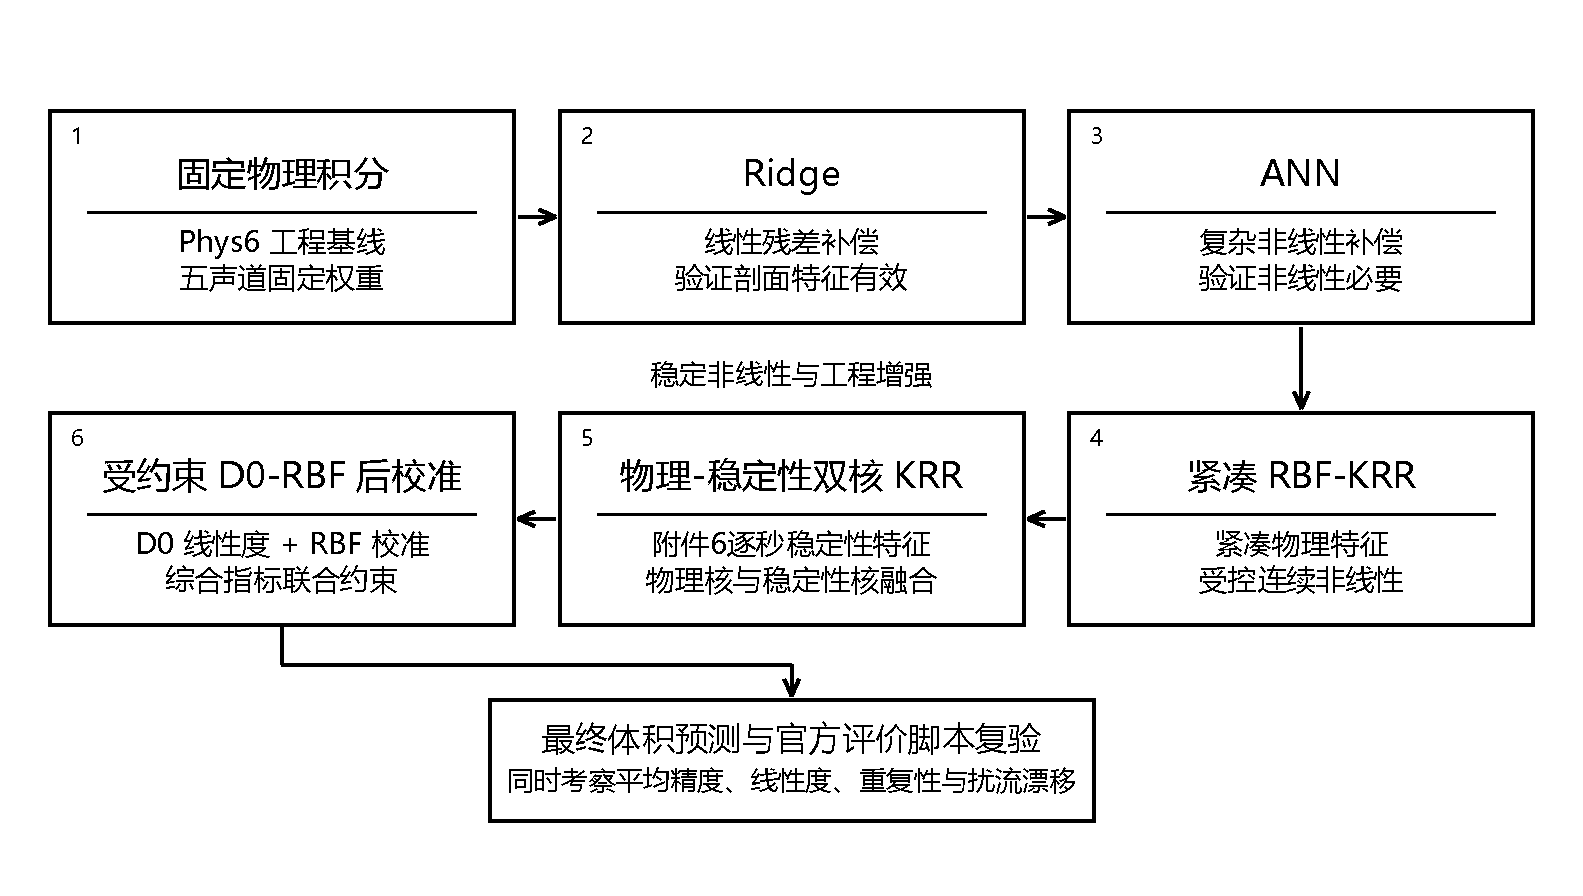
\includegraphics[width=0.98\textwidth]{../figures/fig_problem4_engineering_pipeline.pdf}
  \caption{问题四模型递进的工程方框图}
  \label{fig:problem4_engineering_pipeline}
\end{figure}

除全量拟合基准外，Ridge、ANN 与 KRR 均采用相同的标签盲划分，其中 $118$ 个窗口构成训练集，$41$ 个窗口构成验证集。划分过程按 $h=(\mathrm{date},\mathrm{flow\ point},\mathrm{disturbance\ id})$ 保持重复单元覆盖；日期、窗口编号和人工扰流编号不作为模型输入，特征标准化参数、D0 校准曲线及模型系数均由训练集估计。评价指标包括窗口 MAE、按 $g=(\mathrm{date},\mathrm{flow\ point})$ 构成的评价组、$\max_g|\bar e_g|$ 以及 $u_{\mathrm{nor},L}$、$u_{\mathrm{nor},r}$、$u_{\mathrm{nor},d}$。

\noindent{\circlednumberfont ①}全量拟合基准\par

为检验现有运行时变量对标签的最大表达能力，本文以 Lagrange 体积为基线，将流量尺度、声道、剖面、动态、零点及其平方项和部分交互项扩展为 $358$ 个多项式特征，用带极小正则项的线性模型学习相对修正：
\begin{equation}
\begin{aligned}
r_i
&=\frac{V_i^{\mathrm{std}}}{V_{\mathrm{Lag},i}}-1,\\
\hat V_i
&=V_{\mathrm{Lag},i}
\left(1+\boldsymbol\beta^{\mathsf T}\boldsymbol\phi_i\right).
\end{aligned}
\end{equation}
其中 $\boldsymbol\phi_i$ 为多项式特征，正则化参数为 $\lambda=10^{-9}$。问题一中 Phys6 与 Lagrange 的总体 MAE 分别为 $0.180653\%$ 和 $0.183613\%$，而两者的平均误差分别为 $-0.136424\%$ 和 $-0.007930\%$。为估计高维残差映射的样本内表达上限，本节采用平均偏差较小的 Lagrange 作为近插值基线；泛化模型仍采用总体 MAE 较低的 Phys6。该模型使用全部 $159$ 个窗口的标签进行估计，但运行时输入不含日期、窗口编号、标准体积和人工扰流编号。样本内 MAE 为 $4.777272\times10^{-9}\%$，分组通过率为 $30/30$，$\max_g|\bar e_g|=7.116282\times10^{-9}\%$、$u_{\mathrm{nor},L}=3.861649\times10^{-10}\%$、$u_{\mathrm{nor},r}=2.296923\times10^{-8}\%$、$u_{\mathrm{nor},d}=2.337046\times10^{-8}\%$。

\begin{sloppypar}
改用按日期留一并重新拟合后，MAE 上升到 $0.510512\%$，最大绝对误差更达到 $11.800204\%$。近零的样本内误差没有延续到未见日期，说明高自由度近插值才是其主要来源。即使数据驱动补偿本身已有应用依据\cite{Zhao2014ANN,Li2023MLInUse}，但小样本建模还需要物理约束来限制不合理外推\cite{Cai2025PhysConstrainedGAN}。所以本文只把该模型看作表达能力上限，不让它参与泛化模型的最终选择。
\end{sloppypar}

\noindent{\circlednumberfont ②}Ridge线性残差模型\par

Ridge 先被用来回答一个较简单的问题：紧凑物理特征能否在线性层面解释误差。统一验证集上的 Phys6 基线 MAE 为 $0.179991\%$，只有 $2/7$ 个组通过；此时 $u_{\mathrm{nor},L}$、$u_{\mathrm{nor},r}$ 和 $u_{\mathrm{nor},d}$ 分别为 $0.462931\%$、$0.079400\%$、$0.217668\%$。

加入线性残差后，MAE 降到 $0.091290\%$，分组通过数增加为 $3/7$，扰流综合指标也降至 $0.085595\%$。这些变化说明剖面特征确实含有补偿信息。不过，$u_{\mathrm{nor},L}=0.046127\%$，$u_{\mathrm{nor},r}=0.080151\%$，仍未达到阈值。正常流量曲线、组内波动与扰流附加偏差显然无法由一个线性映射同时描述。

\noindent{\circlednumberfont ③} ANN 非线性残差路线\par

为检验残差关系的非线性特征，本文建立了一隐层 ANN 对照模型。已有研究已将 ANN、机器学习误差预测和 BP 神经网络用于多路径超声流量计的数据融合与误差补偿\cite{Zhao2014ANN,Li2023MLInUse,HuangClampOnOil}。该模型以平均系统偏差较小的 Lagrange 估计量为基线，并输入 $47$ 个运行时特征，以考察高维状态变量的非线性表达能力。ANN 学习百分数相对残差，其监督目标为
\begin{equation}
r_i=100\left(\frac{V_i^{\mathrm{std}}}{V_{\mathrm{Lag},i}}-1\right),
\end{equation}
其中 $r_i$ 的单位为百分数。ANN 预测残差与体积估计写为
\begin{equation}
\begin{aligned}
\hat r_i
&=\boldsymbol{w}_2^{\mathsf T}
\tanh\left(W_1\tilde{\boldsymbol{x}}_i+\boldsymbol{b}_1\right)+b_2,\\
\hat V_i
&=V_{\mathrm{Lag},i}\left(1+\frac{\hat r_i}{100}\right).
\end{aligned}
\end{equation}
式中 $\tilde{\boldsymbol{x}}_i$ 是标准化后的运行时特征。网络只设置一个隐藏层，含 $16$ 个神经元；$L_2$ 系数取 $0.001$，学习率为 $0.01$，共训练 $10000$ 轮。

在同一 $118/41$ 标签盲划分下，ANN 将验证集 MAE 降至 $0.070924\%$，最大组均值绝对值为 $0.147747\%$，分组通过数为 $3/7$。然而，$u_{\mathrm{nor},L}=0.066138\%$、$u_{\mathrm{nor},r}=0.078277\%$，均未随 MAE 一起改善；$u_{\mathrm{nor},d}$ 为 $0.090823\%$。高维运行时变量中确有非线性信息，但窗口平均误差变小，并不等于组内稳定性同步提高。

本题仅有 $159$ 个窗口，而 ANN 输入特征数为 $d=47$，一隐层参数量约为
\begin{equation}
P=(d+1)h+(h+1)=785,
\end{equation}
该参数量显著高于 $118$ 个训练窗口，也远高于有效重复组数量，模型自由度与样本规模不匹配。此外，窗口级均方误差目标不能直接约束最坏组 $SD_g$、$u_{\mathrm{nor},r}$ 和 $u_{\mathrm{nor},d}$，随机初始化和高维输入还会增加估计结果的波动。由此可知，非线性残差建模是必要的，但需要更多样本空间以及进一步压缩特征维度并加强正则化约束。

\subsection{泛化推荐KRR结构}

Ridge 难以同时刻画正常流量曲线、组内重复性和扰流附加偏差，ANN 又受到小样本和高维参数空间的限制。综合来看，模型设计的重点不应继续增加非线性自由度，而应在保留必要非线性表达能力的同时压缩输入空间、强化物理基线并提高求解稳定性。因此，我们采用带正则化的 RBF-KRR，将补偿解释为相似剖面状态之间的连续加权，其基本结构写为
\begin{equation}
\boxed{
\begin{aligned}
\hat V_i
&=V_{\mathrm{Phys6},i}
\left[
1+\frac{
\delta_{\mathrm{KRR}}^{(\%)}(\boldsymbol{x}_i)+
c_{0,\mathrm{post}}^{(\%)}(q_i)}{100}
\right]
\end{aligned}
}.
\label{eq:final_krr_model}
\end{equation}
其中 $V_{\mathrm{Phys6},i}$ 为固定权重工程积分基线，$\boldsymbol{x}_i$ 为问题三构造的紧凑物理特征，$\delta_{\mathrm{KRR}}^{(\%)}$ 为 RBF-KRR 估计的 Phys6 总百分数残差，$c_{0,\mathrm{post}}^{(\%)}$ 为 D0 窗口上的残余校准曲线。两个修正量均以百分数表示。

模型输入由 $15$ 个紧凑物理特征构成，见表~\ref{tab:final_features}。这些特征描述流量尺度、径向剖面、上下不对称、A/B 方向差、动态稳定性、零点漂移以及不同积分规则的相对分歧；标准化参数由训练集估计。表中 $\bar c=(c_0+c_1+c_2+c_3+c_4)/5$。

\begingroup
\scriptsize
\begin{longtable}{p{0.29\textwidth}p{0.25\textwidth}p{0.30\textwidth}c}
\caption{RBF-KRR 的紧凑物理输入特征}
\label{tab:final_features}\\
\toprule
特征 & 计算公式或来源 & 物理含义 & 标准化 \\
\midrule
\endfirsthead
\toprule
特征 & 计算公式或来源 & 物理含义 & 标准化 \\
\midrule
\endhead
$q,\ q^2$ & $(\mathrm{flow\ point}-50)/30$ 及平方 & 归一化流量尺度与二次流量曲线项 & 是 \\
\texttt{profile\_top\_bottom} & 附件剖面字段 & 上下声道差，刻画上下偏流或非对称 & 是 \\
\texttt{profile\_center\_all} & 附件剖面字段 & 中心声道相对整体均值差，刻画中心高速核或中心亏损 & 是 \\
\texttt{profile\_edge\_inner} & 附件剖面字段 & 边缘声道与内侧声道差，刻画近壁梯度变化 & 是 \\
\texttt{profile\_ab\_abs} & 附件剖面字段 & A/B 方向差绝对汇总，刻画传播方向不对称 & 是 \\
\texttt{profile\_swirl} & 附件剖面字段 & 旋流或偏流代理 & 是 \\
\texttt{chord\_center\_minus}\newline\texttt{edges\_frac} & $\bigl(c_2-\frac{c_0+c_4}{2}\bigr)/\bar c$ & 中心--边缘相对差 & 是 \\
\texttt{chord\_edge\_minus}\newline\texttt{inner\_frac} & $\bigl(\frac{c_0+c_4}{2}-\frac{c_1+c_3}{2}\bigr)/\bar c$ & 边缘--内侧相对差 & 是 \\
\texttt{chord\_top\_bottom\_frac} & $(c_0-c_4)/\bar c$ & 上下声道相对差 & 是 \\
\texttt{ab\_abs\_mean} & A/B 差绝对值均值 & A/B 平均绝对差 & 是 \\
\texttt{dyn\_plateau\_cv} & 附件动态字段 & 平台段变异系数，刻画窗口内流量稳定性 & 是 \\
\texttt{zero\_rate\_med} & 附件零点字段 & 零点速率中位数，刻画零点漂移水平 & 是 \\
\texttt{lagrange\_volume\_m3\_minus}\newline\texttt{phys6\_frac} & $(V_{\mathrm{Lag}}-V_{\mathrm{Phys6}})/V_{\mathrm{Phys6}}$ & Lagrange 与 Phys6 相对差，刻画积分方法分歧 & 是 \\
\texttt{owics\_volume\_m3\_minus}\newline\texttt{phys6\_frac} & $(V_{\mathrm{OWICS}}-V_{\mathrm{Phys6}})/V_{\mathrm{Phys6}}$ & OWICS 与 Phys6 相对差，刻画积分方法分歧 & 是 \\
\bottomrule
\end{longtable}
\endgroup

令 $\boldsymbol{z}_i$ 为标准化后的特征向量，RBF 核岭回归残差为\cite{Scholkopf2002LearningKernels}
\begin{equation}
\delta_{\mathrm{KRR}}^{(\%)}(\boldsymbol{x})
=\sum_{j=1}^{n}\alpha_j
\exp\left[-\gamma\|\boldsymbol{z}-\boldsymbol{z}_j\|^2\right].
\end{equation}
训练目标写为
\begin{equation}
\begin{aligned}
\min_{\boldsymbol{\alpha}}\quad&
\left\|\boldsymbol r-K\boldsymbol{\alpha}\right\|_2^2
+\lambda\boldsymbol{\alpha}^{\mathsf T}K\boldsymbol{\alpha},\\
K_{ij}={}&\exp\left[-\gamma\|\boldsymbol z_i-\boldsymbol z_j\|^2\right].
\end{aligned}
\end{equation}
其中 $\boldsymbol r$ 为训练集中相对于 Phys6 基线的总百分数残差：
\begin{equation}
r_i=100\left(\frac{V_i^{\mathrm{std}}}{V_{\mathrm{Phys6},i}}-1\right).
\end{equation}
KRR 初步预测后，再在训练集 D0 窗口上计算残余误差
\begin{equation}
e_i^{\mathrm{raw}}
=100\frac{
V_{\mathrm{Phys6},i}\left[1+
\delta_{\mathrm{KRR}}^{(\%)}(\boldsymbol{x}_i)/100\right]
-V_i^{\mathrm{std}}}{V_i^{\mathrm{std}}},
\end{equation}
并用
\begin{equation}
\begin{aligned}
c_{0,\mathrm{post}}^{(\%)}(q_i)
&\approx -e_i^{\mathrm{raw}},\\
i&\in D0.
\end{aligned}
\end{equation}
拟合二次 D0 后校准曲线。程序中先计算 KRR 初步预测的百分数误差，再以 D0 窗口负误差为目标拟合后校准曲线，与上述公式完全一致。该曲线以标准体积为误差分母，仅修正 KRR 预测后残留的正常工况偏差；KRR 层学习 Phys6 总残差，D0 层学习 KRR 后残余误差，两层职责不同，不构成重复补偿。给定 $\gamma$ 和 $\lambda$ 后，该正则化问题的解为
\begin{equation}
\boldsymbol{\alpha}=(K+\lambda I)^{-1}\boldsymbol r.
\end{equation}
经训练集网格搜索确定
\begin{equation}
\begin{aligned}
\gamma&=0.1,\\
\lambda&=0.1.
\end{aligned}
\end{equation}
在线计算只读取运行时可获得的物理特征。标准体积与标准流量属于标签，日期和窗口编号用于组织样本，工况说明、扰流编号及扰流角度用于离线分析；这些字段都不会进入预测向量。

验证时，D0 曲线、标准化参数和 KRR 系数均在训练集内求得，随后直接作用于验证集。待模型结构和超参数冻结后，才允许用全部标定窗口重估部署参数，用来衡量标定拟合效果。

RBF-KRR 的搜索范围为 $\gamma\in\{0.1,0.3\}$、$\lambda\in\{0.1,1.0\}$，Ridge 与 ANN 提供对照。筛选时先看超限指标的数量，再比较归一化超限程度；若前两项接近，才使用验证集 MAE 排序。最终选取 $(\gamma,\lambda)=(0.1,0.1)$。它在候选配置中最均衡，但并非所有指标都已过线。

表~\ref{tab:ann_krr_compare} 给出两条非线性补偿路线在同一 $118/41$ 标签盲划分下的结果。ANN 采用 Lagrange 基线和 $47$ 个运行时特征，KRR 采用 Phys6 基线、D0 后校准和 $15$ 个紧凑物理特征。因此，表中差异反映物理基线、特征构造和回归方法的综合影响。

\begin{table}[H]
\centering
\caption{ANN 与 RBF-KRR 的同划分验证结果}
\label{tab:ann_krr_compare}
\scriptsize
\begin{tabular}{@{}lccccccc@{}}
\toprule
模型路线 & MAE & 分组 & $\max|\bar e_g|$ & $u_{\mathrm{nor},L}$ & $u_{\mathrm{nor},r}$ & $u_{\mathrm{nor},d}$ & 超限项 \\
\midrule
ANN 对照路线 & 0.070924 & 3/7 & 0.147747 & 0.066138 & 0.078277 & 0.090823 & 3 \\
RBF-KRR 路线 & 0.055176 & 3/7 & 0.159304 & 0.024645 & 0.064035 & 0.083017 & 2 \\
\bottomrule
\end{tabular}
\par\smallskip
{\footnotesize 注：除“分组”和“超限项”外，其余指标单位均为 \%。}
\end{table}

同划分结果表明，ANN 能够识别运行时状态与计量残差之间的非线性关系；RBF-KRR 进一步降低了 MAE、无扰流线性度、重复性和扰流综合指标，超限项数由 $3$ 项减至 $2$ 项。RBF-KRR 的最大组均值绝对值为 $0.159304\%$，略高于 ANN 的 $0.147747\%$，两者均满足 $0.2\%$ 阈值。综合各项指标，RBF-KRR 的平衡性较好。

为检验泛化推荐 KRR 各组成部分的作用，本文在同一标签盲划分上开展四级消融，结果列于表~\ref{tab:krr_ablation}。Phys6 单独预测时，正常工况线性度与扰流综合指标均明显超限。

\begin{figure}[H]
  \centering
  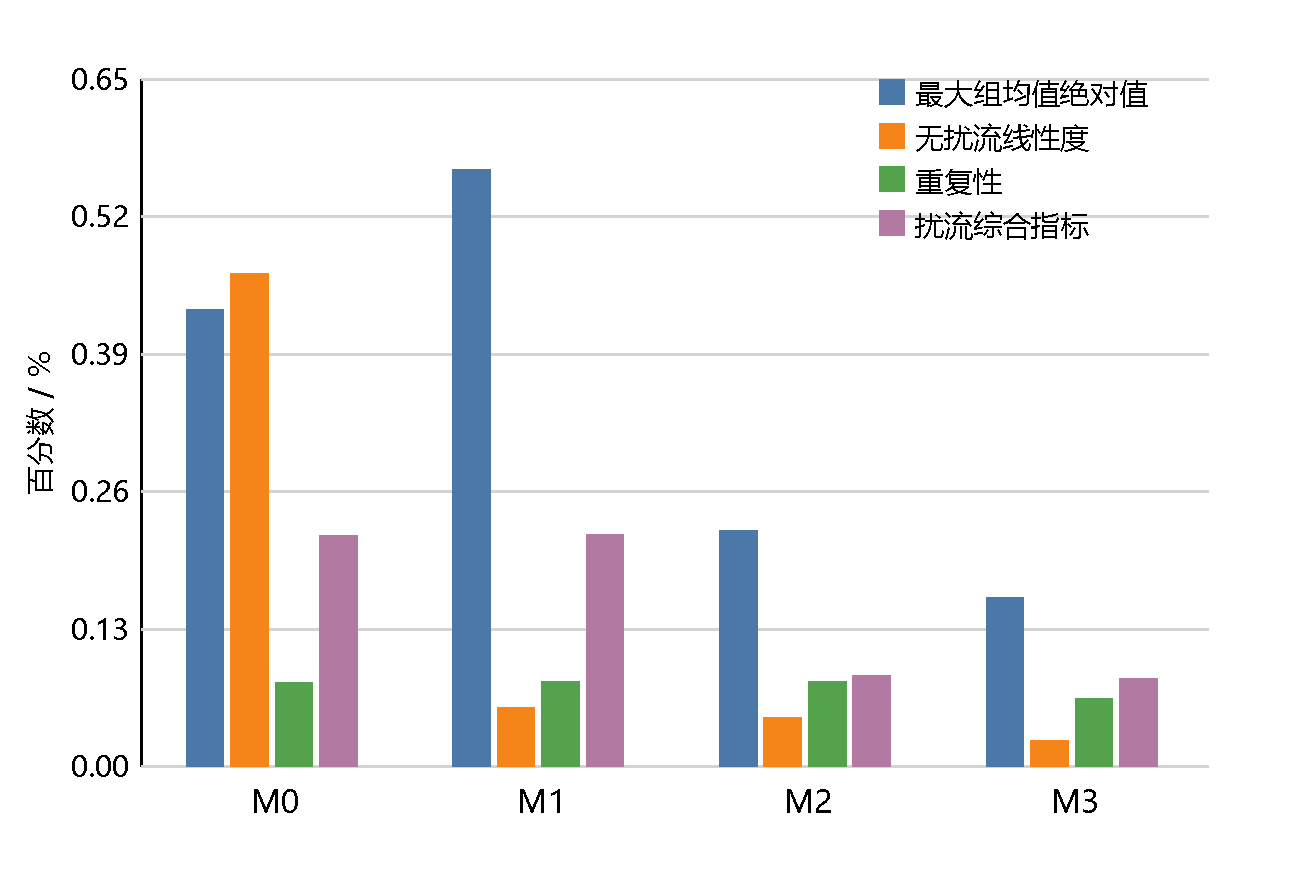
\includegraphics[width=0.70\textwidth]{../figures/fig_krr_ablation_metrics.pdf}
  \caption{四级消融模型与关键指标对比}
  \label{fig:krr_ablation}
\end{figure}

D0 曲线加入后，$u_{\mathrm{nor},L}$ 从 $0.462931\%$ 降至 $0.055310\%$。这表明正常锚点能够修正流量相关偏差，但该曲线并不知道扰流剖面发生了什么，因而 MAE 反而升到 $0.260279\%$，$u_{\mathrm{nor},d}$ 也几乎没有变化。

紧凑特征进入 Ridge 后，MAE 降为 $0.091290\%$，$u_{\mathrm{nor},d}$ 降为 $0.085595\%$。换用 RBF-KRR，MAE 继续下降至 $0.055176\%$，$u_{\mathrm{nor},L}$ 与 $u_{\mathrm{nor},d}$ 均跨过达标线，超限项只剩 $2$ 项。改善来自各层的接续作用，不能只归因于核回归算法本身。

\begin{table}[H]
\centering
\caption{最终主线四级消融结果}
\label{tab:krr_ablation}
\scriptsize
\setlength{\tabcolsep}{3.8pt}
\renewcommand{\arraystretch}{0.92}
\begin{tabular}{lcccccc}
\toprule
阶段 & MAE(\%) & 分组通过 & $u_{\mathrm{nor},L}$(\%) & $u_{\mathrm{nor},r}$(\%) & $u_{\mathrm{nor},d}$(\%) & 超限项 \\
\midrule
Phys6 & 0.179991 & 2/7 & 0.462931 & 0.079400 & 0.217668 & 5 \\
Phys6 + D0 曲线 & 0.260279 & 1/7 & 0.055310 & 0.079728 & 0.218491 & 5 \\
+ Ridge 线性残差 & 0.091290 & 3/7 & 0.046127 & 0.080151 & 0.085595 & 4 \\
+ RBF-KRR & 0.055176 & 3/7 & 0.024645 & 0.064035 & 0.083017 & 2 \\
\bottomrule
\end{tabular}
\end{table}

在主分层标签盲验证中，RBF-KRR 模型取得
\begin{equation}
\mathrm{MAE}=0.055176\%.
\end{equation}
关键达标指标为
\begin{equation}
\max_g|\bar e_g|=0.159304\%\le 0.2\%,
\end{equation}
\begin{equation}
\begin{aligned}
u_{\mathrm{nor},L}&=0.024645\%<0.036\%,\\
u_{\mathrm{nor},r}&=0.064035\%>0.040\%.
\end{aligned}
\end{equation}
\begin{equation}
u_{\mathrm{nor},d}=0.083017\%<0.115\%.
\end{equation}
该模型的平均精度、最大组均值误差、无扰流线性度和扰流综合指标均满足要求，但最大组内重复性超过阈值，评价组通过率为 $3/7$。因此，RBF-KRR 在该划分下具有较好的综合性能，组内重复性是它的主要限制。

\begin{figure}[H]
  \centering
  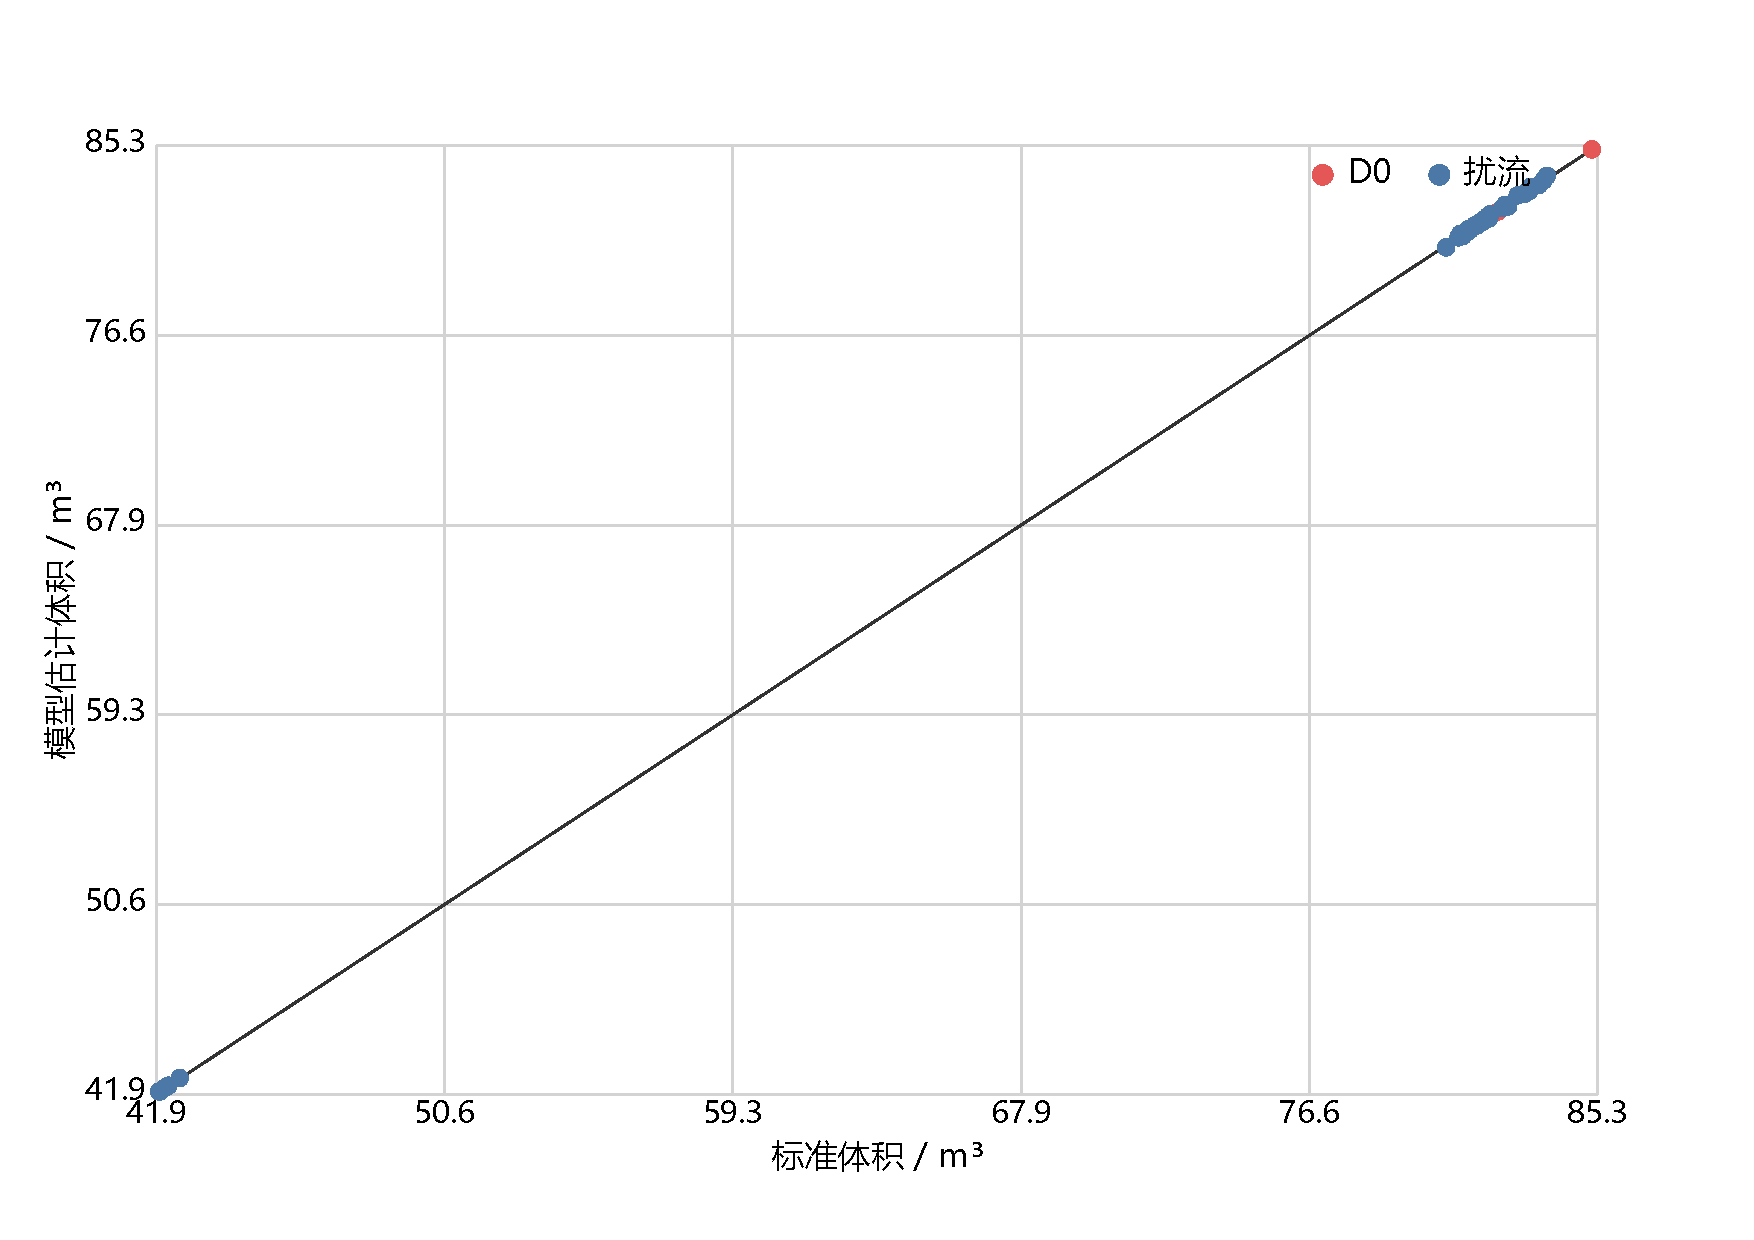
\includegraphics[width=0.70\textwidth]{../figures/fig_prediction_consistency.pdf}
  \caption{RBF-KRR 验证集预测体积与标准体积的一致性}
  \label{fig:prediction_consistency}
\end{figure}

图~\ref{fig:prediction_consistency} 中大部分样本分布在理想一致线附近，说明模型对体积主尺度和系统偏差的控制较好，且未出现明显的整体方向性偏移。然而，散点接近一致线只能反映窗口级预测精度，不能替代同日期、同流量点评价组的重复性检验。$u_{\mathrm{nor},r}=0.064035\%$ 的超限表明，当前紧凑特征仍没有充分解释少数组内的短时状态变化，这也是后续引入逐秒稳定性特征的直接原因。

\subsection{最终推荐模型：双核 KRR 与受约束后校准}

RBF-KRR 的平均误差和扰流漂移已有明显改善，但最坏组重复性仍超过阈值。以附件 6 的逐秒原始声道序列为基础，我们进一步构造物理--稳定性双核 KRR。物理核由紧凑物理特征生成，稳定性核由时差相对离散度、漂移、同步相关、Hampel 异常值替换率、声道波动和 A/B 不匹配等特征生成。两个核按
\begin{equation}
\begin{aligned}
K_{\mathrm{DK}}
&=(1-\beta)K_{\mathrm{physical}}+\beta K_{\mathrm{stab}},\\
K_{\mathrm{physical}}
&=\exp(-\gamma_p d_p^2),\\
K_{\mathrm{stab}}
&=\exp(-\gamma_s d_s^2).
\end{aligned}
\end{equation}
组合，其中 $K_{\mathrm{stab}}$ 表示逐秒稳定性特征核，$\gamma_p=0.05$、$\gamma_s=0.005$、$\beta=0.5$、$\lambda=0.3$。该结构采用 Sch\"olkopf 与 Smola 提出的核正则化思想\cite{Scholkopf2002LearningKernels}。Sakhavi 和 Nouri 的研究表明，多声道速度剖面需要采用独立特征描述\cite{Sakhavi2022GeneralizedProfile}；Li 等的自适应去噪研究说明，窗口内离散度与漂移能够反映观测稳定性\cite{Li2025VMDDenoising}。据此，本文分别构造物理核与稳定性核并进行加权融合。对 $38$ 组候选参数在 $40$ 个按 $h$ 分层的标签盲划分上进行评价，依据超限项数、归一化超限程度、MAE 和分组通过率的中位数确定上述参数。在 $40$ 个划分中，该配置均未实现全部指标同时达标；完整 $159$ 个窗口的样本内 MAE 为 $0.056596\%$，分组通过率为 $13/30$，$u_{\mathrm{nor},L}=0.038713\%$、$u_{\mathrm{nor},r}=0.114864\%$、$u_{\mathrm{nor},d}=0.166680\%$。附件 6 特征增强了窗口稳定性的描述能力，但还不足以控制最坏组重复性。为进一步平衡线性度、重复性和扰流综合指标，本文在双核 KRR 上建立受约束 D0-RBF 后校准层。

最终模型首先按确定的双核参数在完整标定集上重新估计 $\hat V_i^{(\mathrm{DK})}$，随后增加受约束校准层。紧凑特征中的流量尺度记为 $q_i^{(c)}=(\mathrm{flow\ point}_i-50)/30$，D0 线性度曲线采用中心化尺度 $q_i^{(L)}=(\mathrm{flow\ point}_i-70)/30$。最终模型为
\begin{equation}
\begin{aligned}
\hat V_i^{(\mathrm{PC})}
&=\hat V_i^{(\mathrm{DK})}
\left[1+\frac{\Delta_i^{(\mathrm{PC})}}{100}\right],\\
\Delta_i^{(\mathrm{PC})}
&=\mathrm{clip}\left(
\ell(q_i^{(L)})+\rho f_{\mathrm{RBF}}(\boldsymbol z_i),
-0.80,\ 0.80
\right).
\end{aligned}
\label{eq:postcalibrated_dual_kernel_model}
\end{equation}
其中 $\ell(q_i^{(L)})$ 为 D0 正常窗口拟合的线性度校准曲线，$f_{\mathrm{RBF}}$ 为紧凑物理特征与逐秒稳定性特征共同构成的 RBF 校准函数，$\rho$ 为收缩系数。修正幅度限制为 $\pm0.80\%$。固定双核 KRR 结构后，共比较 $5$ 种 D0 曲线、$3$ 组运行时特征、$5$ 个核宽度、$6$ 个正则化系数和 $3$ 个收缩系数，形成 $1350$ 个受约束候选。依据工程阈值通过情况、分组失败数、超限程度、修正幅度和 MAE，确定核宽度 $\gamma=0.1$、正则化系数 $\lambda=0.01$、收缩系数 $\rho=0.75$，并采用线性 D0 校准曲线。

表~\ref{tab:model_evolution_postcalibrated} 汇总各阶段结果。其中，标签盲验证用于评价模型对未参与训练窗口的预测能力，同样本全量标定用于估计给定标定窗口的拟合效果，两种评价口径分别列示。

\begin{table}[H]
\centering
\caption{模型演进与全量标定结果比较}
\label{tab:model_evolution_postcalibrated}
\scriptsize
\setlength{\tabcolsep}{2.5pt}
\begin{tabular}{p{0.20\textwidth}p{0.16\textwidth}cccccc}
\toprule
阶段 & 评价口径 & MAE & 分组 & $\max|\bar e_g|$ & $u_{\mathrm{nor},L}$ & $u_{\mathrm{nor},r}$ & $u_{\mathrm{nor},d}$ \\
\midrule
高维多项式近插值 & 159窗口样本内 & $4.78\!\times\!10^{-9}$ & 30/30 & $7.12\!\times\!10^{-9}$ & $3.86\!\times\!10^{-10}$ & $2.30\!\times\!10^{-8}$ & $2.34\!\times\!10^{-8}$ \\
ANN 对照 & 标签盲验证 & 0.070924 & 3/7 & 0.147747 & 0.066138 & 0.078277 & 0.090823 \\
紧凑 KRR & 标签盲验证 & 0.055176 & 3/7 & 0.159304 & 0.024645 & 0.064035 & 0.083017 \\
物理--稳定性双核 KRR & 159窗口样本内 & 0.056596 & 13/30 & 0.088743 & 0.038713 & 0.114864 & 0.166680 \\
受约束 D0-RBF 后校准双核 KRR & 同样本全量标定 & 0.015891 & 30/30 & 0.028735 & 0.009585 & 0.033630 & 0.048435 \\
\bottomrule
\end{tabular}
\par\smallskip
{\footnotesize 注：除“分组”外，其余指标单位均为 \%。}
\end{table}

由表~\ref{tab:model_evolution_postcalibrated} 可知，高维多项式模型的样本内误差最低，但留一日期误差明显增大；ANN 能够刻画非线性残差，但在小样本条件下稳定性不足；紧凑 RBF-KRR 和物理--稳定性双核 KRR 提高了模型的物理可解释性与窗口稳定性描述能力，最坏组重复性仍是主要限制。受约束 D0-RBF 后校准双核 KRR 在全量标定数据上进一步平衡线性度、重复性和扰流漂移，用于生成最终体积估计。其数值反映给定标定窗口的拟合效果，未知日期和扰流状态仍需通过独立数据检验。

问题三的聚类结果显示，D1--D8 在在线特征空间中没有形成稳定的多类边界；$K=2$ 时主要将 D3 单独分出，其余扰流状态仍大量重叠。硬聚类专家会把前级错分继续传递到体积估计，因此本文采用统一 RBF-KRR 对局部相似剖面连续加权。最终体积估计使用受约束 D0-RBF 后校准双核 KRR，适用于题目给定的标定窗口；新增日期或未知扰流状态需由独立样本重新评价。

\subsection{结果分析}

模型演进表明，误差均值下降并不等于工程指标同步改善。紧凑 RBF-KRR 在标签盲验证中的 MAE 为 $0.055176\%$，无扰流线性度和扰流综合指标分别为 $0.024645\%$ 与 $0.083017\%$，均已满足阈值；但重复性为 $0.064035\%$，评价组仅通过 $3/7$，说明少数组内短时变化仍未被充分描述。

加入逐秒稳定性信息后，双核结构能够把剖面差异与窗口波动分开度量，但在完整标定样本内仍只有 $13/30$ 个评价组通过。进一步采用受约束无扰流后校准后，题目给定 $159$ 个标定窗口上的 MAE 降为 $0.015891\%$，分组通过率为 $30/30$，三项综合指标分别为 $0.009585\%$、$0.033630\%$ 和 $0.048435\%$。

上述结果对应两种不同证据。标签盲划分反映模型对未参与训练窗口的预测能力，而后校准双核 KRR 的全部达标结果属于同样本全量标定，只能说明其适合生成题目给定窗口的最终体积估计。对新增日期或未知扰流状态，仍需固定特征、核参数和校准形式后使用独立数据复验。

\section{灵敏度与失效分析}

\subsection{校准、残差与聚类敏感性}

四级消融表明，D0 曲线主要影响无扰流线性度：
\begin{equation}
u_{\mathrm{nor},L}: 0.462931\%\longrightarrow 0.055310\%.
\end{equation}
加入该曲线后，MAE 由 $0.179991\%$ 增至 $0.260279\%$，$u_{\mathrm{nor},d}$ 未同步改善。无扰流校准能够修复正常工况的流量相关偏差，但结果依赖 D0 锚点的覆盖范围。

在线剖面特征进入 Ridge 后，MAE 为 $0.091290\%$，$u_{\mathrm{nor},d}=0.085595\%$，说明线性模型已能解释部分扰流附加偏差；此时 $u_{\mathrm{nor},L}=0.046127\%$、$u_{\mathrm{nor},r}=0.080151\%$，仍超过阈值。RBF-KRR 将 MAE 降至 $0.055176\%$，并得到 $u_{\mathrm{nor},L}=0.024645\%$、$u_{\mathrm{nor},r}=0.064035\%$、$u_{\mathrm{nor},d}=0.083017\%$。物理--稳定性双核 KRR 加入逐秒稳定性特征后，标签盲划分中的最坏组重复性仍未达标。核映射对平均误差和扰流漂移较为有效，而重复性更依赖局部样本覆盖。

扰流聚类采用 KMeans、Ward 和对角 GMM，并令 $K=2,\ldots,5$。最高 Silhouette 系数为 $0.377676$，出现在 $K=2$ 的 KMeans；一个簇主要对应 D3，其余扰流编号大量重叠，系统漂移型与重复性失稳型也没有形成清晰边界。聚类数变化没有改变这一判断，因此使用统一 RBF-KRR 的连续相似性补偿。

\subsection{整组留出、OOD 与失效诊断}

普通分层验证会在同一 $h$ 单元内同时保留训练窗口和验证窗口。为模拟新日期或新工况，压力测试把完整重复单元
\begin{equation}
h=(\mathrm{date},\mathrm{flow\ point},\mathrm{disturbance\ id}),
\end{equation}
移出训练集，并用 $SD_h$ 记录留出单元内部的误差波动。$SD_h$ 只用于失效诊断，不替代官方按 $g=(\mathrm{date},\mathrm{flow\ point})$ 计算的 $SD_g$ 与 $u_{\mathrm{nor},r}$。压力测试未能实现全部指标同时达标。

在紧凑物理标准化特征空间中，最近邻 OOD 距离定义为
\begin{equation}
d_{\mathrm{OOD}}(x_i)=\min_{j\in \mathcal{T}}
\left\|\boldsymbol z_i-\boldsymbol z_j\right\|_2,
\end{equation}
其中 $\mathcal{T}$ 为训练窗口集合。保留全部压力测试组时，MAE 与 OOD 距离的 Pearson 相关系数为 $0.910943$，Spearman 系数仅为 $0.078788$。极端组 \texttt{20260607-60-D0} 的 OOD 距离达到 $54.8812$；删除该点后，Pearson 系数变为 $-0.305248$。高线性相关主要由正常锚点完整缺失驱动，普通扰流组的误差不能只由 OOD 距离解释。

\begin{figure}[!htbp]
  \centering
  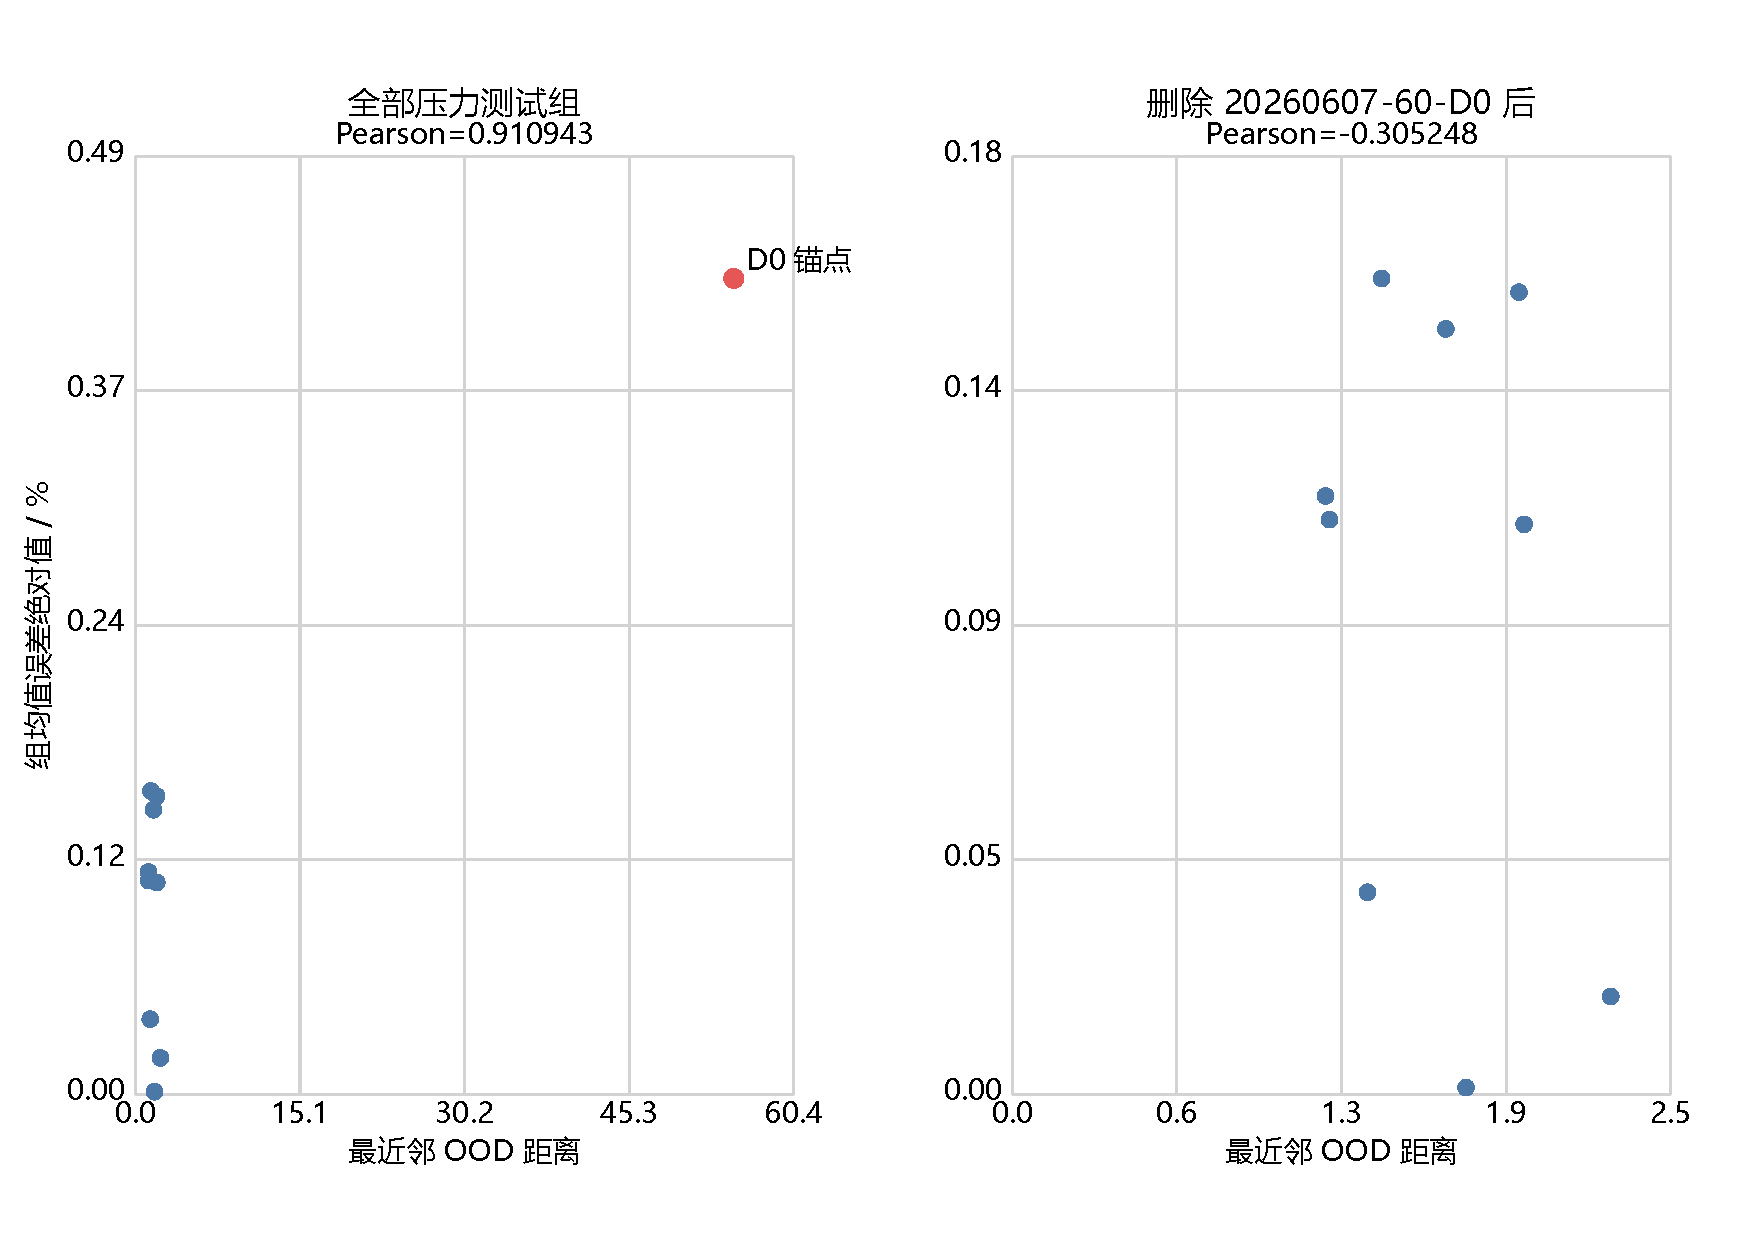
\includegraphics[width=0.92\textwidth]{../figures/fig_krr_ood_vs_error.pdf}
  \caption{压力测试全部组及删除极端 D0 锚点后的 OOD--误差关系}
  \label{fig:krr_ood}
\end{figure}

表~\ref{tab:failure_mechanisms} 将压力测试误差归纳为三类。正常锚点缺失表现为组内波动较小而均值偏差显著；扰流系统漂移表现为特定方向性扰流下的稳定偏差；重复性失稳则具有较小均值误差和较大的 $SD_h$，与窗口内短时剖面变化有关。

\begin{table}[!htbp]
\centering
\caption{整组留出压力测试的三类失效机制}
\label{tab:failure_mechanisms}
\scriptsize
\begin{tabular}{p{0.16\textwidth}p{0.22\textwidth}p{0.22\textwidth}p{0.26\textwidth}}
\toprule
失效类型 & 代表性工况 & 主要诊断量 & 机理解释 \\
\midrule
正常锚点缺失型 & \texttt{20260607-60-D0} & OOD 距离 $54.8812$，$|\bar e|=0.423406\%$，$SD=0.022659\%$ & 组内波动较小而均值偏差显著，属于正常标定锚点缺失引起的系统外推 \\
扰流系统漂移型 & \texttt{20260609-60-D5}；\texttt{20260613-60-D4} & $|\bar e|$ 分别为 $0.154697\%$、$0.115376\%$ & 特定方向性扰流产生稳定偏差，统一补偿函数仍有局部欠拟合 \\
扰流重复性失稳型 & \texttt{20260608-60-D7}；\texttt{20260615-60-D2} & 均值偏差相对较小，但单元内 $SD_h$ 超过 $0.040\%$ & 短时剖面或动态状态变化未被现有紧凑特征完全描述 \\
\bottomrule
\end{tabular}
\end{table}

图~\ref{fig:leave_one_group_heatmap} 给出逐组留出条件下扰流编号与流量点的平均误差，较大偏差集中在少数扰流与流量组合。

\begin{figure}[H]
  \centering
  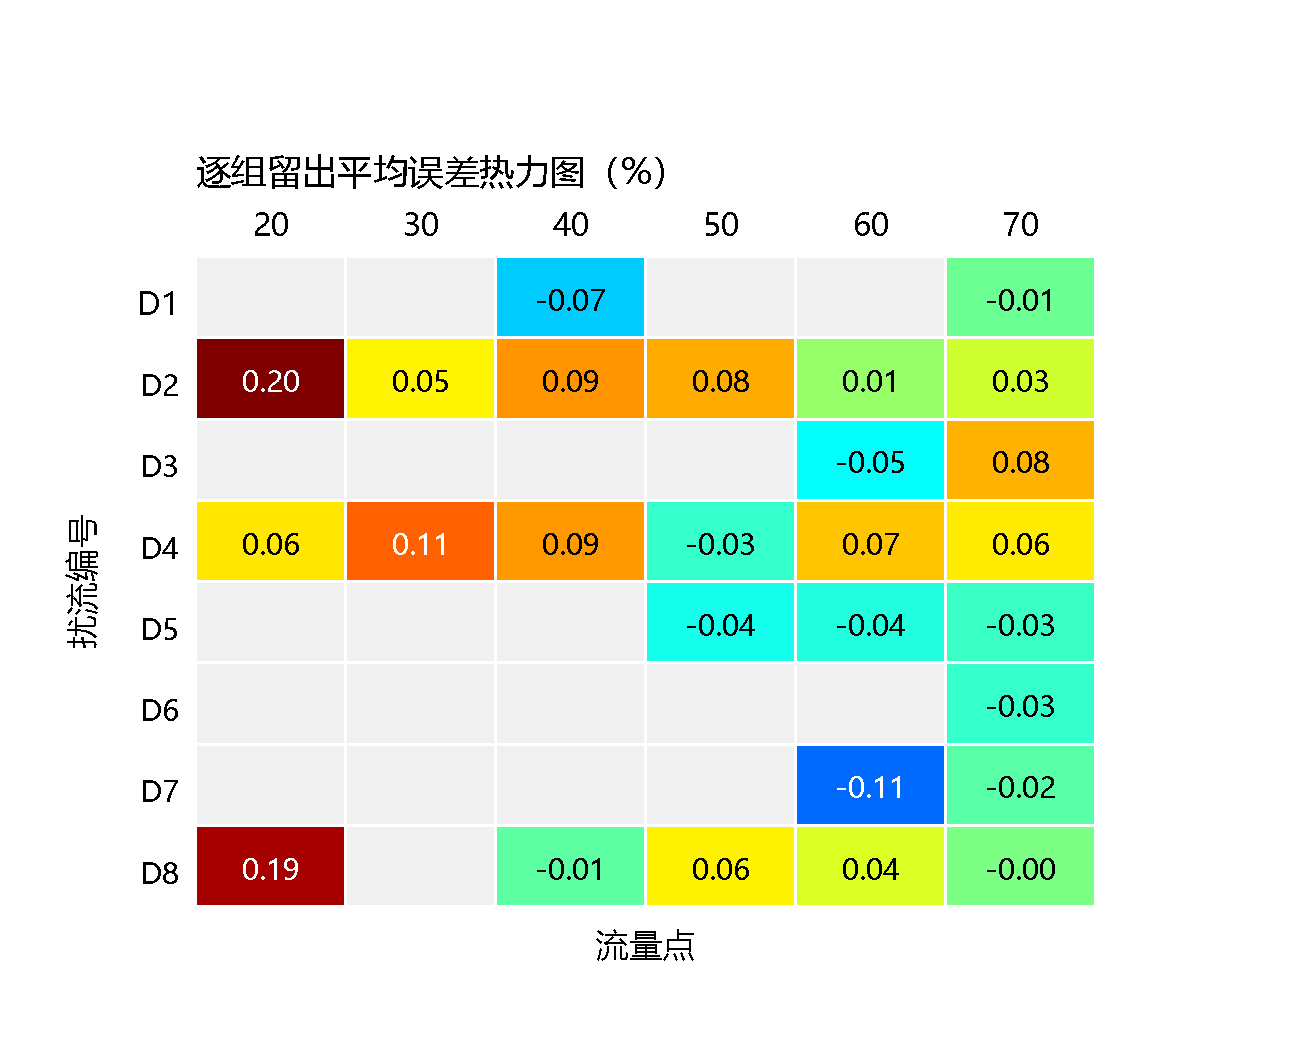
\includegraphics[width=0.78\textwidth]{../figures/fig_leave_one_group_error_heatmap.pdf}
  \caption{逐组留出平均误差热力图}
  \label{fig:leave_one_group_heatmap}
\end{figure}

\section{模型评价与推广}

\subsection{模型优点}

所建模型包括泛化基线和全量标定模型两个层次。泛化基线以传播时间差和 Phys6 工程积分估计量为物理基础，利用紧凑物理特征与 RBF-KRR 学习相对于 Phys6 的总百分数残差，并通过 D0 窗口平滑校准正常工况的残余误差。进一步引入附件 6 的逐秒稳定性特征，形成物理核与稳定性核加权的双核 KRR；最终模型在确定的双核参数基础上重新估计全量标定模型，并增加受约束 D0-RBF 后校准层。

与 ANN 和高维多项式模型相比，紧凑 KRR 与物理--稳定性双核 KRR 的特征维数较低，物理含义较为明确。聚类结果表明，除 D3 外，多数扰流状态在在线特征空间中连续重叠，统一核补偿与该数据结构相适应。在标签盲划分中，紧凑 KRR 的 MAE 为 $0.055176\%$，$u_{\mathrm{nor},L}$ 和 $u_{\mathrm{nor},d}$ 满足阈值，而 $u_{\mathrm{nor},r}$ 没有达标。双核 KRR 引入逐秒稳定性特征后，全量样本内评价的分组通过率为 $13/30$，重复性仍然是主要限制。

$40$ 个标签盲随机分层划分中，物理--稳定性双核 KRR 的窗口平均精度较为稳定，但未出现全部指标同时通过的划分，主要瓶颈是最坏组重复性。因此，该模型适合作为当前数据条件下具有物理解释的泛化基线。在此基础上构造的受约束 D0-RBF 后校准双核 KRR，经题设评价程序复验得到 MAE $0.015891\%$、分组通过率 $30/30$、$u_{\mathrm{nor},L}=0.009585\%$、$u_{\mathrm{nor},r}=0.033630\%$、$u_{\mathrm{nor},d}=0.048435\%$，给定标定窗口上的各项指标均满足阈值。

\subsection{模型局限}

模型的主要局限在于完整未见工况的外推能力。压力测试显示，正常工况锚点或扰流重复组完全缺失时，模型可能产生系统漂移或重复性失稳。其中，\texttt{20260607-60-D0} 属于正常锚点缺失型 OOD，D5、D4 的部分工况表现为扰流系统漂移，D7、D2 的部分工况表现为组内重复性失稳。因此，实际应用还需同时监测组均值误差、组内 SD 和 OOD 距离。后校准双核 KRR 的达标结果对应给定 $159$ 个标定窗口，其未知工况性能仍需独立数据验证。

D1--D8 为离线实验条件编号，在当前在线特征空间中未形成稳定可分的流型类别。“硬聚类专家模型”是先将窗口唯一判定为某个扰流簇，再调用该簇的独立补偿器；当簇边界重叠时，分类错误会直接传递到流量估计。“软门控补偿”则不作唯一分类，而是根据窗口与各状态中心的相似度产生连续权重，对多个补偿器的输出加权融合。现有样本不足以稳定训练上述多专家结构，因此两者均未用于当前后校准双核 KRR。样本进一步扩充后，可将软门控作为研究方向。

\subsection{推广方向}

模型可从三个方面推广。其一，增加 D0 正常流量点和跨日期无扰流样本，以提高 D0 后校准曲线 $c_{0,\mathrm{post}}^{(\%)}(q)$ 的锚点覆盖；其二，针对系统漂移型扰流构造连续的剖面漂移补偿，避免依赖人工扰流编号；其三，针对重复性失稳型扰流引入更细的窗口内动态稳定性指标和局部平滑约束，以降低 $SD_g$。若能够获得原始回波信号，可采用自适应去噪改善时差估计\cite{Li2025VMDDenoising}；样本扩充后还可比较物理约束数据增强方法\cite{Cai2025PhysConstrainedGAN}，并利用独立真实工况检验生成样本的有效性。实际部署时应记录模型版本、标准化参数、OOD 距离和组内重复性，用于长期漂移诊断与现场复标。

\subsection{AI 工具使用说明}

我们在图表排版和文字校对阶段使用了 ChatGPT 5.6Sol 辅助工具\cite{OpenAICodex2026}。所有建模公式、评价指标口径、实验代码和数值结论均由作者结合题面、附件数据和官方评价脚本逐项核对；AI 输出只作为辅助建议，不直接替代人工判断。详细使用场景、采纳内容和人工修改说明见随文提交的《AI工具使用详情.pdf》。


\referencescn
\ifdefined\WordExport
\else
  \newpage
  \appendixcn
\fi

\end{document}
